\documentclass[11pt]{article}

\usepackage{deauthor,times,graphicx}
\graphicspath{{submissions/grade-sql-chandra/figs}}
%\usepackage[hidelinks]{hyperref}
\usepackage{hyperref} 

%%%%%%%%%%%%%%%%%%%%%%%%%%%%%%%%%%%%%
\newcommand{\smalltt}[1]{{{\texttt{#1}}}}
\newcommand{\paras}[1]{\noindent\textit{#1}:}
\newcommand{\tabsql}{\hspace*{3mm}}
%%%%%%%%%%%%%%%%%%%%%%%%%%%%%%%%%%%%%

\newcommand\blfootnote[1]{%
  \begin{NoHyper}%
  \renewcommand\thefootnote{}\footnote{#1}%
  \addtocounter{footnote}{-1}%
  \end{NoHyper}%
}

\begin{document}
\title{Automated Grading of SQL Queries}
\author{Bikash Chandra*\blfootnote{Currently at Meta Platforms Inc.} \hspace{1cm} S. Sudarshan \\ IIT Bombay \\ \texttt{\{bikash,sudarsha\}@cse.iitb.ac.in}}
\maketitle

%%%%%%%%%%%%%%%%%%%%%%%%%%%%%%%%%%%%%%%
\begin{abstract}
In a traditional classroom setting, instructors and teaching assistants either grade SQL queries either manually or using fixed datasets. Manual grading is tedious, error-prone and does not scale well for courses with a large number of students or for online courses. Using fixed datasets may miss even common errors and mark incorrect student queries as correct. In this article, we discuss our system XData that, given a set of correct queries, can automatically evaluate the correctness of SQL queries using datasets designed to catch errors in the given correct queries. If a student query is found to be incorrect, XData can even assign grades to the query based on how close they are to a correct query. In our experience, these techniques can be used to grade queries for settings with a large number of students with little human effort and involvement. 
\end{abstract}

\section{Introduction}
\label{seC:intro}
% Interpretability and nutritional labels, generally

An essential ingredient of successful machine-assisted decision-making, particularly in high-stakes decisions, is interpretability --– allowing humans to understand, trust and, if necessary, contest, the computational process and its outcomes.   These decision-making processes are typically complex:  carried out in multiple steps, employing models with many hidden assumptions, and relying on datasets that are often repurposed --- used outside of the original context for which they were intended.\footnote{See Section 1.4 of Salganik's ``Bit by Bit''~\cite{salganik} for a discussion of data repurposing in the Digital Age, which he aptly describes as "mixing readymades with custommades.''}  In response, humans need to be able to determine the ``fitness for use'' of a given model or dataset, and to assess the methodology that was used to produce it.  

To address this need, we propose to develop interpretability and transparency tools based on the concept of a {\em nutritional label}, drawing an analogy to the food industry, where simple, standard labels convey information about the ingredients and production processes. Short of setting up a chemistry lab, the consumer would otherwise have no access to this information. Similarly, consumers of data products cannot be expected to reproduce the computational procedures just to understand fitness for their use.   Nutritional labels, in contrast, are designed to support specific decisions by the consumer rather than completeness of information.  A number of proposals for hand-designed nutritional labels for data, methods, or both have been suggested in the literature\cite{DBLP:journals/corr/abs-1803-09010,DBLP:journals/corr/abs-1805-03677,DBLP:conf/fat/MitchellWZBVHSR19}; we advocate deriving such labels automatically or semi-automatically as a side effect of the computational process itself, embodying the paradigm of {\em interpretability-by-design}. 

Interpretability means different things to different stakeholders, including individuals being affected by decisions, individuals making decisions with the help of machines, policy makers, regulators, auditors, vendors, data scientists who develop and deploy the systems, and members of the general public.  Designers of nutritional labels must therefore consider {\em what} they are explaining,  {\em to whom}, and {\em for what purpose}.  In the remainder of this section, we will briefly describe two regulatory frameworks that mandate interpretability of data collection and processing to members of the general public, auditors, and regulators,  where nutritional labels offer a compelling solution (Section~\ref{sec:intro:reg}).  We then discuss interpretability requirements in data sharing, particularly when data is altered to protect privacy or mitigate bias (Section~\ref{sec:intro:synth}).

\subsection{Regulatory Requirements for Interpretability}
\label{sec:intro:reg}

The European Union recently enacted a sweeping regulatory framework known as the General Data Protection Regulation, or the GDPR~\cite{gdpr}.  The regulation was adopted in April 2016, and became enforceable about two years later, on May 25, 2018.  The GDPR aims to protect the rights and freedoms of natural persons with regard to how their personal data is processed, moved, and exchanged (Article 1).  The GDPR is broad in scope, and applies to ``the processing of personal data wholly or partly by automated means'' (Article 2), both in the private sector and in the public sector.  Personal data is broadly construed, and refers to any information relating to an identified or identifiable natural person, called the {\em data subject} (Article 4).  

According to Article 4, lawful processing of data is predicated on the data subject's {\em informed consent}, stating whether their personal data can be used, and for what purpose (Articles 6, 7).
Further,  data subjects have {\em the right to be informed} about the collection and use of their data.~\footnote{\url{https://gdpr-info.eu/issues/right-to-be-informed/}}
Providing insight to data subjects about the collection and use of their data requires technical methods  that support interpretability.  

Regulatory frameworks that mandate interpretability are also starting to emerge in the US.  New York City was the first US municipality to pass a law (Local Law 49 of 2018)~\cite{Vacca}, requiring that a task force be put in place to survey the current use of ``automated decision systems'' (ADS) in city agencies. ADS are defined as ``computerized implementations of algorithms, including those derived from machine learning or other data processing or artificial intelligence techniques, which are used to make or assist in making decisions.''   The task force is developing recommendations for enacting algorithmic transparency by the agencies, and will propose procedures for: (i) requesting and receiving an explanation of an algorithmic decision affecting an individual (Section 3 (b) of Local Law 49); (ii) interrogating ADS for bias and discrimination against members of legally protected groups, and addressing instances in which a person is harmed based on membership in such groups (Sections 3 (c) and (d)); (iii) and assessing how ADS function and are used, and archiving the systems together with the data they use (Sections 3 (e) and (f)).

Other government entities in the US are following suit.  Vermont is convening an Artificial Intelligence Task Force to ``... make recommendations on the responsible growth of Vermont’s emerging technology markets, the use of artificial intelligence in State government, and State regulation of the artificial intelligence field.''~\cite{Vermont}.  Idaho’s legislature has passed a law that eliminates trade secret protections for algorithmic systems used in criminal justice~\cite{Idaho}.  In early April 2019, Senators Booker and Wyden introduced the Algorithmic Accountability Act of 2019 to the US Congress~\cite{BookerWydenClarke}. The Act, if passed, would use ``automated decision systems impact assessment'' to address and remedy harms caused by algorithmic systems to federally protected classes of people. The act empowers the Federal Trade Commission to issue regulations requiring larger companies to conduct impact assessments of their algorithmic systems.

The use of nutritional labels in response to these and similar regulatory requirements can benefit a variety of stakeholders.  The designer of a data-driven algorithmic method may use them to validate assumptions, check legal compliance, and tune parameters.  Government agencies may exchange labels to coordinate service delivery, for example when working to address the opioid epidemic, where  at least three sectors must coordinate: health care, criminal justice, and emergency housing, implying a global optimization problem to assign resources to patients effectively, fairly and transparently. The general public may review labels to hold agencies accountable to their commitment to equitable resource distribution. 


\subsection{Interpretability with Semi-synthetic Data}
\label{sec:intro:synth}

%Datasets are now increasingly used to train models to make decisions once made by humans.  In these automated systems, biases in the data are propagated and amplified with no human in the loop.  The bias, and the effect of the bias on the quality of decisions made, is not easily detectable due to the relative opacity of the system.  

A central issue in machine-assisted decision-making is its reliance on historical data, which often embeds results of historical discrimination, also known as {\em structural bias}.   As we have seen time and time again, models trained on data will appear to work well, but will silently and dangerously reinforce discrimination~\cite{propublicaJ,amazon_hiring,amazon_delivery}.  Worse yet, these models will legitimize the bias --- ``the computer said so.''  Nutritional labels for data and models are designed specifically to mitigate the harms implied by these scenarios, in contrast to the more general concept of ``data about data.''

Good datasets drive research: they inform new methods, focus attention on important problems, promote a culture of reproducibility, and facilitate communication across discipline boundaries.  But research-ready datasets are scarce due to the high potential for misuse. Researchers, analysts, and practitioners therefore too often find themselves compelled to use the data they have on hand rather than the data they would (or should) like to use.  For example, aggregate usage patterns of ride hailing services may overestimate demand in early-adopter (\ie wealthy) neighborhoods, creating a feedback loop that reduces service in poorer neighborhoods, which in turn reduces usage.  In this example, and in many others, there is a need to alter the input dataset to achieve specific properties in the output, while preserving all other relevant properties.  We refer to such altered datasets as \textit{semi-synthetic}.

Recent examples of methods that produce semi-synthetic data include database repair for causal fairness~\cite{DBLP:conf/sigmod/SalimiRHS19}, database augmentation for coverage enhancement~\cite{DBLP:conf/icde/AsudehJJ19}, and privacy-preserving and bias-correcting data release~\cite{DBLP:conf/ssdbm/PingSH17,DBLP:conf/vldb/RodriguezSPSH18}. A semi-synthetic datasets may be altered in different ways.  Noise may be added to it to protect privacy, or statistical bias may be removed or deliberately introduced.  When a dataset of this kind is released, its composition and the process by which it was derived must be made interpretable to a data scientist, helping determine fitness for use.  For example, datasets repaired for racial bias are unsuitable for studying discrimination mitigation methods, while datasets with bias deliberately introduced are less appropriate for research unrelated to fairness.   This gives another compelling use case for nutritional labels.

%To make our discussion more concrete, let us consider data scientists who must identify datasets appropriate for their task.  This is particularly important when semi-synthetic datasets are being released, to which noise is added to protect privacy, or statistical bias is removed or deliberately introduced.  For example, datasets repaired for racial bias are unsuitable for studying discrimination mitigation methods, while datasets with bias deliberately introduced are less appropriate for research unrelated to fairness.  



\section{Using Datasets to Check Correctness}
\label{sec:datagen}
Test data generation in XData is done based on the correct queries provided by the instructor. Unlike fixed datasets that are query agnostic, these datasets are designed to catch errors based on the correct queries provided by the instructor and are hence much better at catching errors. 

\subsection{Common Errors in SQL Queries}
Students make several types of errors when writing SQL queries. Some students may use an inner join when a left outer join was required, others may use a count aggregation when a count distinct was needed. Mutation testing is a well-known approach to check the adequacy of test cases for a program~\cite{mutation}. We use a similar approach for mutation testing of SQL queries.  We consider mutations as (syntactically correct) changes to an SQL query. Errors made by student queries may be seen as mutations of the correct query and the incorrect query is called a non-equivalent mutant of the correct query. A dataset that produces different results on the correct and incorrect queries is said to kill the mutation. 

XData produces multiple datasets. The first dataset is aimed to produce a non-empty result for the query. This dataset itself kills several mutations. For the remaining datasets, XData considers single mutations at a time on the correct query provided by the instructor and generates datasets that are targeted to kill the mutations. Each dataset is marked with a tag to indicate which type of mutations a dataset is designed to catch. Note that a dataset designed to catch one type of mutation may catch other types of mutations as well. 

XData considers a large number of mutations in SQL queries including but not limited to the following.
\begin{itemize}
    \item \textbf{Join type mutation}: A join type mutation involves replacing one of \smalltt{\{INNER, LEFT OUTER, RIGHT OUTER\} JOIN} with another.  Since the same join query may be written using different join orders, XData considers mutations across different join orders. Mutations involving missing or additional join orders are also considered. 
%XData nullifies each join condition separately.

    \item \textbf{Selection predicate mutation}: For selection conditions, XData considers mutations of the relational
operator where any occurrence of one of  \{$=, <>, <, >, \leq, \geq$\} is replaced by another or if the selection condition is missing. XData also considers mutations of selection predicates between \texttt{IS NULL} and \smalltt{NOT IS NULL} and for missing \smalltt{IS NULL}. These predicates may be on integer, floating, text attributes or even aggregates. Mutations involving changing the constant in the selection condition are also considered. 
    \item \textbf{Aggregation mutation}: Aggregations may be either unconstrained (at the root of the query tree) or constrained (having a condition with the aggregate). In both cases, the aggregation function can be mutated among \smalltt{MAX, MIN, SUM, AVG, COUNT} and their \smalltt{DISTINCT} versions. 
    Mutations involving \smalltt{COUNT(attr)} to \smalltt{COUNT(*)}, in case \smalltt{attr} is nullable, are also considered. 
    \item \textbf{Group by attribute mutation}: For queries involving the \smalltt{GROUP BY} clause, XData considers mutations involving additional or missing group by attributes both in the presence and absence of the \smalltt{HAVING} clause. 
    \item \textbf{Like operator mutation}: Like operators are used in SQL to match patterns in text attributes. SQL like operators include \smalltt{LIKE, NOT LIKE, ILIKE and NOT ILIKE}. XData considers mutation of any one SQL like operator to other like operators. XData also considers mutations in the patterns used with the LIKE operator such as replacing as '\%' with '\_' and vice versa or missing '\%' or '\_' in the pattern.
    \item \textbf{Nested subquery mutations}: XData considers mutations between \smalltt{IN} $vs.$ \smalltt{NOT IN}, \smalltt{EXISTS} $vs.$ \smalltt{NOT EXISTS} and \smalltt{ALL} $vs.$ \smalltt{ANY/SOME}. Mutations on the queries in the nested subquery are also considered for test data generation so that errors inside subqueries are also caught. 
    \item \textbf{Set operator mutations}: Set operators are used in compound queries to combine the results of two underlying results. Set operator mutations include changing one of the following operators to another: \smalltt{UNION, UNION ALL, INTERSECT, INTERSECT ALL, EXCEPT, EXCEPT ALL}. Similar to nested subqueries, mutations of the subqueries whose results are input to these set operators are also considered. 
    \item \textbf{Distinct mutation}: Duplicates in the results may be filtered using the \smalltt{DISTINCT} clause. XData considers mutations of a missing or extraneous \smalltt{DISTINCT} clause.
\end{itemize}

\subsection{Test Data Generation to Detect Errors}
For each type of mutation, we design specific conditions that the datasets must satisfy in order to kill such mutations. Let us take the following example query to demonstrate the mutations considered for queries with join and selections and how we generate datasets to kill the mutations.

\smalltt{\tabsql SELECT course.course\_id\\
\tabsql FROM course INNER JOIN takes USING(course\_id)\\
\tabsql WHERE course.credits >= 6}

Some of the mutations that XData would consider and the techniques to kill those are the following. 

\begin{enumerate}
\item \textbf{Join type mutation}: Consider the
mutation from department INNER JOIN course to
department LEFT OUTER JOIN course. In order to
kill this mutation, we need to ensure that there is a
tuple in department relation that does not satisfy the
join condition with any tuple in course relation. The
INNER JOIN query would not output that tuple in
the department relation while the LEFT OUTER
JOIN would.

In general, a join query can be specified in a join order
independent fashion, with many equivalent join orders for a given query. Hence, the number of join type
mutations across all these orders is exponential. From
the join conditions specified in the query, XData
forms equivalence classes of $<$relation, attribute$>$
pairs such that elements in the same equivalence
class need to be assigned the same value to meet
(one or more) join conditions. Using these equivalence
classes, XData generates a linear number of datasets
to kill join type mutations across all join orderings.
If a pair of relations involve multiple join conditions
\item \textbf{Selection Predicate mutation}: For killing mutations for the selection condition A1 relop A2, XData
generates 3 datasets where tuples satisfy the conditions (1) A1 $>$ A2, (2) A1 $<$ A2,
and (3) A1 $=$ A2. These three datasets kill all non-
equivalent mutations from one relop to another relop. These datasets also kill mutations because of missing
selection conditions. 

For the given query example the constraints would be (1) \smalltt{course.credits>6}, (2) \smalltt{course.credits<6} and (3) \smalltt{course.credits=6}. If the student query uses a different operator instead of $>=$ or misses the selection condition one of the three datasets will catch the error.
\end{enumerate}

Details on test data generation for killing other types of mutations are presented in \cite{xdata:vldbj15}. We omit the details here for brevity. 

It is not sufficient for only the conditions for killing mutations to be satisfied when generating the test database. The difference at one level, say the join condition must change the result of the query for the difference to be observed in the query result. For the given example query, consider the join mutation. If all tuples in course have grade less than 6, both the \smalltt{INNER JOIN} and the \smalltt{LEFT OUTER JOIN} would give empty results. Hence, when generating a dataset, XData ensures that the tuple has \smalltt{grade >= 6}. 

In order to generate a dataset, we generate constraints using an SMT solver~\cite{smt}. In XData, we support CVC3~\cite{CVC3}, CVC4~\cite{CVC4} as well as Z3~\cite{z3} as the constraint solvers. We encode text attributes as enumerates types and enumerates types are modeled as subtypes of integers or rationals. A tuple type is created for each relation to represent one row and an array of tuples represents the relation table. We also add other database constraints such as primary key and foreign key constraints, unique attribute constraints as well as domain constraints. The domain constraints ensure that we generate the correct types of values for each column of the database, the values generated are within the range specified by the schema and only nullable columns can have NULL values.



We also note that some mutations may be semantically equivalent to the correct queries and it may not be possible to kill such mutations. For such cases, the constraints for killing the mutations would not be satisfiable and the SMT solver would fail to generate the dataset to kill the mutation.

For the given query, a simplified version of the constraints, to generate the dataset that produces a non-empty result would be as follows (assuming none of the columns are nullable).
\begin{verbatim}
%Data definition
DATATYPE course_id = CS-101 | BIO-301 | CS-312 | PHY-101 END;
credits:TYPE = SUBTYPE (LAMBDA (x: INT): x > 1 AND x < 11);
course_tuple_type:TYPE = [course_id,credits];
course: ARRAY INT OF course_tuple_type;

%Primary key constraints
ASSERT FORALL(i:course_index, j:course_index): 
       course[i].0 = course[j].[0] => course[i].1 = course[j].1

%Foreign key constraints
ASSERT FORALL(i: takes_index):
       EXISTS (j: course_index): takes[i].1 = course[j].0;

%Query conditions
ASSERT course[1].0 = takes[1].1;
ASSERT course[1].1 >= 6;
\end{verbatim}

To support nullable columns, we add additional values (outside the domain of the column) for the datatype that correspond to NULL values and explicitly mark those as NULL values. 
Also, in practice, we found that unfolding the constraints (i.e., specifying the constraints for each tuple instead of FORALL, NOT EXISTS) gives us much better performance~\cite{xdata:icde11}. We decide the number of tuples upfront and assert the constraint on each tuple. 

\subsection{Evaluating Correctness of Student Queries}
The dataset generation for each correct query is done once across all students. Based on the datasets generated, XData compares the results of each student query and each correct query provided by the instructor. If all results of the student query are found to match that of a correct query, the student query passes that correct query.

When an instructor specifies multiple correct queries, XData allows the instructor to specify one of the two options 
\begin{itemize}
    \item The additional queries were added to provide more coverage and better testing and all correct queries are equivalent. The student query will need to pass all correct queries for it to be marked as correct. 
    \item The question test provided by the instructor was ambiguous and there could be multiple interpretations of the correct result. In this case, the student query will be marked correct if it passes any one of the correct queries. 
\end{itemize}

The XData system ensures that student queries are safely executed on a different database using temporary tables to ensure that their queries do not interfere with the main database or that the queries of one evaluation do not interfere with another. 


\section{Edit Based Suggestions For Learning}
\label{sec:edit}
Generating test data using correct queries provided by the instructor works great for finding student queries with errors. However, once the query is found to be incorrect, the student should be awarded partial marks based on the extent of correctness. It is also useful to make suggestions to the students so that can understand the errors in their queries. 

One way to award marks for correctness could have been to use the fraction of datasets (generated by XData) that the student query could pass. This approach turns out to be unfair and could penalize small errors heavily while providing a better score to queries that have more errors. Such examples are shown in \cite{xdata:comad}. Another way to grade student queries would be to just check for the differences between the correct query and the student query. However, this approach may deduct more marks than required as explained below.

\subsection{Approach}


The approach we use instead in XData is to compare the student query to each correct query and make changes or edits to the student query to attempt to make it equivalent to the correct query. After each edit, the student query is compared to the correct query  and the changes are stopped once the student query is equivalent to the correct query. 
Checking for equivalence after each edit could have been done using test data generation but that would be very expensive and grading each student query could take minutes. Other approaches for checking equivalence such as Cosette~\cite{cosette} as well as techniques based on tableau~\cite{tableaux1} work on a limited subset of query constructs and were hence not considered.

Marks are deducted based on the required edits. The edits required are also used to suggest what changes the students should have made to their query to make it correct, thereby providing individualized feedback to each student without any additional human involvement. For each type of query construct being edited, the instructor of the course can specify the weight for that edit. For example, for a query where the instructor is evaluating the student's ability to write aggregations correctly, the instructor may want to deduct more marks for errors in aggregation than for other errors. By default, XData assigns equal weight to each edit being considered.

In general, more than one edit may be needed to make the student query equivalent to the correct query. It is important to note that the order in which the edits are made is also important and that is not sufficient to just compare the query trees of the correct query and the student query to find the changes. One edit to a student query may allow us to rewrite other parts of the query in a different way. As an example consider the following pair of queries from Section~\ref{sec:intro}.
\begin{itemize}
    \item Correct query: \smalltt{SELECT * FROM r INNER JOIN s ON (r.A=s.A) WHERE r.A>10}
    \item Student query: \smalltt{SELECT * FROM r INNER JOIN s ON (r.A=s.B) WHERE s.A>10}
\end{itemize}

There are two differences between the student query and the correct query - the selection condition and the join condition. If the student query is graded just based on these differences, marks corresponding to two edits would be deducted. Even if we grade based on the edits required, if the selection condition is edited first, followed by the join condition 2 edits would be required. On the other hand, if the join condition is edited first and the join condition in the student query is changed to \smalltt{r.A=s.A}, the selection condition in the student query becomes equivalent to that of the correct query. 

\subsection{Query Canonicalization}
The student and correct query may be written in different ways. For example, the correct query may use a selection condition \smalltt{A>5} while the student query may write the condition as \smalltt{NOT(A<=5)}. In order to compare the query structure of the student query to the correct query, we need to make them comparable. The student query and the correct query are made comparable by using canonicalizations. 

XData considers two types of canonicalizations:
\begin{itemize}
    \item \textbf{Syntactic Canonicalization}: This is the pre-processing step to reduce irrelevant syntactic differences. These include attribute disambiguation, replacing \smalltt{NOT, BETWEEN, and WITH} constructs and removing \smalltt{ORDER BY} from subqueries. 
    \item \textbf{Semantic Canonicalization}: In this step, based on the query conditions and the database constraints, the queries are canonicalized semantically. Such canonicalizations include but are not limited to removing distinct clauses based on primary key information and converting outer joins to inner joins based on non-nullable foreign key information. 
\end{itemize}
A detailed list of the canonicalizations is provided in ~\cite{xdata:comad}. Such canonicalization rules are often used in query optimizers. However, the goal of the canonicalizations in XData is to get more standard forms of the query.

XData also flattens the query tree where possible (\smalltt{INNER JOIN, UNION(ALL), INTERSECT(ALL)} as well as predicates involving AND or OR).  For the parsed query tree shown in Figure~\ref{fig:parsedTree},  XData would flatten the tree to the one shown in Figure~\ref{fig:flattenedTree}. The flattened tree children are compared in an ordered way for non-commutative operators such as \smalltt{LEFT OUTER JOIN, EXCEPT(ALL)} and \smalltt{ORDER BY} attribute lists while for commutative operators the order of operands is ignored while matching. 


\begin{figure}
	\centering
	\begin{minipage}{0.40\textwidth}
	\centering
	\includegraphics[width=1\textwidth,keepaspectratio=true]{/parsedTree.pdf}
		\caption{Parsed Tree From Query}
		\label{fig:parsedTree}
	\end{minipage}
		\begin{minipage}{0.59\textwidth}
	\centering
	\includegraphics[width=1\textwidth,keepaspectratio=true]{/flattenedTree.pdf}
		\caption{Flattened Tree}
		\label{fig:flattenedTree}
	\end{minipage}
\end{figure}


\subsection{Edit Sequence Based Grading}
XData considers the following form of edits to the flattened tree generated from the student query.
\begin{itemize}
    \item  inserting a node/subtree into the flattened tree
\item removing a node/subtree from the flattened tree
\item replacing an existing node/subtree from a flattened tree
with another node/subtree in the flattened tree
\item moving a node/subtree from one position of the flattened
tree to another
\end{itemize}

When editing a flattened tree generated from a student query, an infinite number of possible edits could be made. However only edits that make the query more similar to the correct query would be useful. In order to add edits that make the student query more similar to the correct query, XData uses the correct query to guide the edits that are generated. The guided edits are based on the differences the student flattened student query tree has with the flattened tree of the correct query. For example, query attributes/conditions/constructs not used in the correct query but present in the student query will be removed when generating edits. 
For each query edit that XData generates, marks corresponding to the edit as configured by the instructor are deducted. The marks deducted for the edit can be considered the edit cost. 

XData can generate multiple guided edits on the student query at each step. From each of these edited queries, more edits are possible. Consider a graph whose nodes are all queries for the given schema. For a student query  SQ, edits of the query are also nodes in the graph. Let these edited queries be connected to query SQ with an edge whose weight is the edit cost of the edited query. Canonically equivalent queries, i.e. their canonical forms are the same, are connected by 0 cost edges. The sequence of edits that has the least cumulative cost can now be determined based on the shortest path in this graph from the student query node in the graph to a correct query node. Partial marks can now be awarded based on this shortest path.  Since the weight of each edge, which represents the cost of edit is non-negative, the shortest possible path may be found using Dijkstra’s shortest path algorithm. Hence, given a set of edits and using a given set of canonicalizations, the shortest path in the graph, as defined above, gives the edit sequence with the least cost.  
We note that the graph discussed above is for the ease of understanding only and XData does not proactively try to generate the entire graph. In practice, XData generates the nodes of the graph on the fly as needed. 

In case the instructor specifies multiple correct queries, the edit sequence based algorithm run based on all correct queries and the best partial marks obtained is awarded. 

\subsection{Heuristic solution}
Even with using only guided edits, the search space is still very large for larger queries if we consider all guided edits to get the shortest path from the student query to the correct query. Hence in practice, we use a greedy heuristic. The heuristic uses a cost benefit model. For each  edited query we can get an estimate of how incorrect the query is by finding the differences between the canonicalized versions of the edited query and the correct query. A weighted sum (based on the weight assigned by the instructor for each edit) can be used to find an edit distance which we call the \textit{canonicalized edit distance}. Each guided edit reduces the canonicalized edit distance to the correct query. The reduction in the canonicalized edit distance from the edit is the benefit of the edit. 

For the heuristic algorithm, at each edit step, we find the $benefit-cost$ for each edit. We then pick the edit that has the highest value of the $benefit-cost$ and use it to generate further edits. The remaining edits are discarded at each step. Using the heuristic allows XData to search a much smaller search space. For the incorrect student queries that we had in our course, we found that the heuristic solution works as well and takes orders of magnitude less time as compared to the exhaustive solution  \cite{xdata:comad}.



\section{Automated Grading Experience}
\label{sec:exp}
We have successfully used the XData automated grading system across several offerings of undergraduate database courses at IIT Bombay. Before using XData in a course, we empirically confirmed, using results from a previous database course, that XData was able to catch as many as or more errors than when the grading was done manually or when fixed datasets are used for grading. This result was consistent across all questions that XData was able to grade. We found, in several cases, that manual grading had missed subtle errors such as a missing distinct clause. 

For the initial course offerings, we used only generated dataset based grading to check for correctness and had to award partial marks manually. The dataset-based grading significantly reduced the human effort involved and allowed us to catch more errors than would have been possible with manual grading.
In several cases, however, students were not satisfied since they could not intuitively understand how marks had been deducted or what the error in their specific query was. The tagged datasets on which the student queries failed were shown but often there would be too many of them to understand the specific error. A dataset designed to catch one type of mutation may catch other types of mutations as well and hence it was not always clear what the actual error was. Several students contested the scores that they had been awarded when their query was found to be incorrect. Awarding partial marks manually by the graders was still tedious since students often wrote queries in very different and complex ways. Manually transforming such student queries to a simpler form was difficult. For instance, in one case a correct query involved using a NOT IN clause and some students used a combination of multiple EXCEPT and INTERSECT clauses.  

When using partial marking in combination with dataset based evaluation, we reduced the human effort as well as provided much better feedback. 
We experienced fewer students contest grades when it was assigned automatically compared to when a human would manually assign grades. The edit-based guidance was also  useful for students to understand where they went wrong. For the first course setting where we used automated partial marking for evaluation, we found that across 1800 student query submissions that were graded by XData, only 2 queries were contested by students. In both cases, we traced back the errors in grade to bugs in our code. One of the main challenges when using automated grading was to provide sufficient types of correct queries that covered the student queries.  

Since the edit sequence based guided edits provide a way to change an incorrect student query to a correct query, the guided edits can be used by students to learn the mistakes that they made and how the mistakes could have been corrected. Such feedback was very helpful especially for beginners to understand how to write correct SQL queries.  
\section{Related Work}
\label{sec:relwork}
There has been a significant interest in testing query equivalence or correctness and in automated grading. Related work include the following.

\subsection*{Checking Query Equivalence}

XData uses test data generation based on mutation testing to generate test datasets to check the equivalence of the correct query and student query. Tuya et al.~\cite{mutation1} describe a number of possible mutations for SQL queries. However, they do not handle test data generation for killing these mutations. Other approaches on testing query equivalence using datasets include Qex~\cite{QEX} and SQL full predicate coverage by Riva et al.~\cite{Riva:2010}. Test data generation in these systems is aimed at testing SQL queries in database applications and they consider only a limited subset of SQL query constructs. 

Techniques based on tableau~\cite{tableaux} and its extensions~\cite{tableaux1, tableaux2} can be used to check for query equivalence for a restricted class of conjunctive queries. Cosette~\cite{cosette} and U-semiring~\cite{semantic} can also be used to check for SQL semantic equivalence using a restricted set of axioms. 
SPES~\cite{spes} uses a symbolic approach for checking query equivalence on SQL queries under bag semantics for select-project-join(SPJ) queries as well as aggregate and union queries. 

\subsection*{Grading SQL Queries}
The Gradiance system~\cite{gradience} provides multiple choice type questions where the instructor has to provide some correct as well as incorrect answers and explanations of incorrectness. In such assignment settings, since the students are only able to select from limited options, subtle mistakes that students could make may not always be covered by the incorrect answers. Gradescope\cite{gradescope}, uses a fixed dataset to evaluate the correctness of student SQL queries. As discussed earlier, using fixed datasets may miss errors and would not be able to provide any meaningful feedback to incorrect student queries. RATest~\cite{rattest} provides feedback for incorrect queries by deriving small datasets that produce different results in a student query as compared to a correct query. I-Rex~\cite{irex} allows users to trace the SQL query evaluation for each constituent block in the query execution. 


\subsection*{Automated Grading for Programming Assignments}
Grading programming assignments has some similar challenges as grading database queries. CPSGrader~\cite{cpsgrader} can grade programming assignments for cyber-physical systems using constraints synthesis and uses reference solutions to provide feedback. AutoGrader~\cite{autograder} can grade introductory level python programs and provide student feedback using program synthesis and high-level error modeling specifications. However, AutoGrader can only model specific predictable errors. 

SARFGEN~\cite{sarfgen} provides feedback to student queries by aligning student programs to similar correct reference programs and finds the minimum number of edits to the student program to match the chosen reference program.  This approach is similar to our approach of edit-based grading. However, SQL queries have database constraints that are not part of the query but need to be accounted for during edits and equivalence checking. Hence we have a more complex semantic canonicalization step that can take into account constraints such as primary keys and foreign keys.





%%%%%%%%%%%%%%%%%%%%%%%%%%%%%%%%%%%%%%%%%
\section{Conclusion and Open Challenges}
\label{sec:conclusion}
The XData system is very useful for grading assignments on SQL queries and for providing feedback to students about mistakes they made. For large classes or online courses, such automated grading systems are essential and the automated individualized feedback would be very useful to new learners. Our experience in using the grading system has been very positive from both the teaching assistants as well as the students. The XData grading system as well as the  source code
are available for download from {\url{http://www.cse.iitb.ac.in/infolab/xdata}}.


One of the key challenges in the XData grading scheme is the number of ways a correct SQL query can be written. We have found that students sometimes write queries using a very different approach than we had anticipated. Catching errors with such approaches as well as awarding partial marks in these cases may be challenging. One way to address these would be to automatically group student query submissions and generate datasets for one student query in each group. We could then use the datasets to identify correct queries from the group and automatically add these as additional correct queries for grading. 
Another key challenge is in dealing with student queries that have additional query constructs that do not affect the query results. One of the cases that we found in our course was when a student had used the query {\smalltt{Q UNION Q'}} where Q' was always empty. The query had one error in Q but marks were also deducted based on edit for Q'.  


\paragraph*{Acknowledgments:} We thank all students and researchers who worked on the XData project as well as those who used the system and provided their valuable feedback. This work was partially supported by research funding and a PhD fellowship from Tata Consultancy Services. 
%%%%%%%%%%%%%%%%%%%%%%%%%%%%%%%%%%%%%%
%\bibliographystyle{IEEEtran}
%\bibliography{references}

\documentclass[11pt]{article} 


%%%%%%%%%%%%%%set margin to 1in

%%%%%%%%%%%%%%%%%%%%

\usepackage{amsmath}
\usepackage{verbatim}
\usepackage{comment} 
\usepackage{algorithm}
\usepackage{algorithmic}
\usepackage{amsfonts}
\usepackage{amssymb}
%\usepackage{amsmath}
\usepackage{subfig}
\usepackage{multirow}
\usepackage{flushend}
\usepackage{caption}
\usepackage{url}
%\usepackage{xspace}
%\usepackage{xcolor}
%\usepackage{enumitem,url}
\usepackage{deauthor,times,graphicx}

\usepackage{bbm}




\newcommand{\ceil}[1]{\left\lceil{#1}\right\rceil}
\newcommand{\floor}[1]{\left\lfloor{#1}\right\rfloor}

\newcommand{\remove}[1]{}

\newcommand{\bbone}{\mathbbm{1}}
\newcommand{\cK}{{\mathcal  K}}
\newcommand{\cS}{{\mathcal  S}}

\newcommand{\degrees}{$\!\!$\char23$\!$}
\DeclareFontFamily{OT1}{psyr}{}
\DeclareFontShape{OT1}{psyr}{m}{n}{<-> psyr}{}
\def\times{{\fontfamily{psyr}\selectfont\char180}}

%\newtheorem{definition}{Definition}
%\newtheorem{example}{Example}
\newtheorem{problem}{Problem}
\newcommand{\hide}[1]{}


\renewcommand{\refname}{\centerline{References}}

% this handles hanging indents for publications
\def\rrr#1\\{\par
\medskip\hbox{\vbox{\parindent=2em\hsize=6.12in
\hangindent=4em\hangafter=1#1}}}

\def\baselinestretch{1.01}

\begin{document}
\title{Fairness and Robustness in Answering Preference Queries}

\author{
Senjuti Basu Roy\\
New Jersey Institute of Technology\\
senjutib@njit.edu}


\date{}

\maketitle
\begin{abstract}

Given a large number of users preferences as inputs over a large number of items, preference queries leverage different preference aggregation methods to aggregate individual preferences in a systematic manner and come up with a single output (top-$k$ ordered or unordered/a complete order) that is most representative. The preference aggregation methods are widely adopted from the social choice theory, some of which are rank based (single-round vs. multi-round), while others are non-rank based. These queries are prevalent in high fidelity applications, including search, ranking and recommendation,  hiring and admission, and electoral voting systems. This article outlines algorithmic challenges and directions in designing an optimization guided computational framework that allows to change the original  aggregated output (either ordered or unordered top-$k$ or a complete order) to satisfy different criteria related to {\em fairness and robustness}, considering different preference elicitation models (ways users provide their input preferences) and aggregation methods (ways the individual preference get aggregated). 


\end{abstract}


\vspace{-0.1in}
\section{Introduction}
\vspace{-0.1in}
The need to aggregate a large number of individual preferences in a  systematic manner is {\em ubiquitous}. Users can provide preferences in many ways - as likes/dislikes, ordinal preferences, or ranked order (full or partial). The social choice theory~\cite{feldman2006welfare} offers a plethora of aggregation methods to aggregate individual preferences and come up with a single output. These outputs may be a single rank that is most representative of all users preferences, or sometimes a smaller number of $k$ items (top-$k$) that are ordered or  presented as a set. While  designed for electoral voting systems primarily, the applicability of answering queries is prevalent in many high fidelity applications, such as, ranking and listing web search results, recommending movies/songs,  selecting a handful of candidates for domains where resource is scarce (such as hiring and admission), to name a few. It is not a stretch to consider a setting in which thousands of items (notationally $n$) have received preferences from hundreds of thousands (or even millions) of users (notationally $m$) and the goal is to produce a single output (notationally $\sigma$) that is most {\em representative}. 



The computational implications of different preference aggregation methods are well studied. {\em What is not so well understood is how hard it is to change the original produced output, which may be necessary for many compelling reasons.}  Satisfying additional criteria, such as, promoting fairness (e.g., ensuring presence of individuals with certain socio-demographic properties),  or Understanding robustness, i.e., figuring out the minimum amount of change of the inputs that would result in a different outcome than the original output. This latter aspect provides understanding on how manipulable the proposed aggregation methods are which are certainly important for aggregation methods that are heavily used in electoral systems, but are applicable in other scenarios as well (e.g., in figuring out the robustness of a rating system of products). To the best of our knowledge, {\em a systematic study is needed to investigate these aspects in conjunction with different preference elicitation models, requiring different preference aggregation methods.} That, in nutshell, is the focus of this article.

%While our focus is studying how to change the original output of the preference aggregation methods that may be necessary for different reasons, 
\smallskip \noindent We discuss these challenges considering four interspersed dimensions, as described below.

\smallskip \noindent {\em \bf Preference Elicitation Models.}
The article simultaneously considers a vast range of preference elicitation processes that we broadly categorize as rank based and non rank based. In rank based processes, the users can provide a fully ranked order over all items, a partial order, or a coarser preference (like item a ranked higher than item b, etc). In non rank based preferences, users can provide only likes, both likes and dislikes, or even an ordinal preference (likes item a as "excellent", b as "good", etc). The choice of these preference elicitation methods is dictated by the different applications. Rank based ones are suitable in hiring/admission/electoral system, while non rank based ones are more relevant in obtaining user feedback from search results, user satisfaction survey, product reviews, etc.

\smallskip \noindent {\em \bf Preference Aggregation Methods.}
Then the preference aggregation methods that are most commensurate to the underlying preference elicitation process and underlying application are studied. For example, when user preferences are given as ranked order, depending on the underlying application, we will aggregate them using existing single-round rank based methods  (e.g., Kemeny, Spearman's footrule, or Borda), or multi-round based methods (STV, IRV). The former aggregation methods are suitable in hiring decision, whereas, the latter ones are gaining popularity in voting systems. On the other hand, when users provide non rank based preferences, we will show how Jaccard similarity or Hamming distances are suitable to aggregate them and come up with the final output. 

\smallskip \noindent {\em \bf Produced Output Form.}
From the application point of view, the produced output may require an order over all $n$ items (hiring/admission), or a small number $k$ of $n$ items as outputs. In case of top-$k$ items requirement, the returned $k$-items may need to be ordered for certain applications  (top-$k$ web pages returned by the search engine), or in some cases it is fine to return them as a set (selecting a set of representatives or body to form certain committee). 

\smallskip \noindent {\em \bf Change Original Output.}
The importance of quantifying the minimum effort needed to change the original output is evident for several reasons, such as  promoting fairness and robustness. Robustness is heavily used in {\em electoral system} to produce {\em margin},  that investigates how to bound the amount of change of the original outcome in case x\% of the inputs are destroyed/deleted/modified. We discuss them further in details below.
%\begin{itemize}
 %   \item {\bf Promoting additional criteria.} It is highly desirable in many compelling applications to produce outputs that satisfy additional criteria (e.g., fairness, diversity) while staying as close as possible to the original output.
  %  \item {\bf Study robustness.} In many practical applications, especially ones related to voting and electoral system, there is a need to understand the following question. How to bound the amount of change of the original outcome in case x\% of the inputs are destroyed/deleted/modified. This problem relates to finding {\em margin} in electoral system, which intends to figure out how much change is needed in the original input to even minimally change the original outputs. 
%\end{itemize}



%\smallskip \noindent {\bf Proposed Project.} 
%The project will be executed based on three broadly defined aims. %The first part of the proposal will study different preference elicitation models of the members , with the objective of producing fairness aware~\cite{zehlike2021fairness,verma2018fairness,chairman, pfair,layard2008social,amer2009group,berkovsky2010group} preference aggregation models. The outcomes of this objective are formalism/models that incorporate fairness with preference aggregation and studies a wide spectrum of variants.  Then, we  focus on the computational aspect of the proposed problems - investigate their hardness, and propose efficient solutions with provable guarantees. Our efficiency consideration shall also investigate how to reuse the current computation if the inputs come dynamically and over time. Finally, we will demonstrate how to enable actionable fair preference aggregation in two compelling applications including electoral voting systems (such as ranked choice voting~\cite{rank1,rank2}) and perform additional experimental evaluation for qualitative and computational efficacy. 

%\smallskip \noindent{Research challenges.}

\vspace{-0.1in}
\section{Overarching Research Goals}
\vspace{-0.1in}
The overarching goal is to design optimization guided computational framework containing principled models and scalable solutions that allows to change the original  aggregated output  (either ordered or unordered top-$k$ or a complete order) to satisfy different criteria, considering different  preference elicitation models and aggregation functions to promote:  \textbf{a.~Fairness} from the standpoint of the protected attributes\cite{verma2018fairness} of the items/candidates  %as well as of the members
(e.g., race, gender, ethnicity), where the candidates are selected by aggregating elicited preferences of the members (panelists, voters, search committee). We shall investigate existing group fairness criteria in the context of preference aggregation~\cite{zehlike2021fairness,verma2018fairness}, as well as adapt fairness criteria studied in the context of resource allocation or social choice theory.  \textbf{b.~Robustness}, namely, understanding how easy or hard it is to change the original outcome of different preference aggregation models given a budgeted preference substitution requirement. For instance, if the total number of preference updates is budgeted to be $\leq x$, is it possible to change the original outcome? 
 We are interested in exploring these viewpoints for multiple preference elicitation models and output forms.  What is also important to notice is that a given preference elicitation may be suitable to multiple aggregation methods and may require to satisfy more than one produced output form. These gives rise to many combinations of the problem.

%Our long term vision is the ambitious goal of developing a computational framework that is flexible enough to accommodate any domain expert defined criteria to minimally change the outcome of any existing preference aggregation protocol to promote additional criteria that are commensurate to new rules and policies, as well as present efficient and automated computations of outcomes.
%To realize these contributions, we propose to develop a computational framework containing a suite of principled models by formalizing multiple ways of changing outcomes of initial preference aggregation solutions considering individual preference elicitation models that are suitable to a wide variety of compelling applications and design efficient solutions for those. 


\smallskip \noindent The rest of the article is organized as follows:
\smallskip \noindent In Section~\ref{aim1}, we study how to Satisfy output constraints in single round rank-based preference aggregation methods.
We study this considering ranking, which is a commonly used method to prioritize  desirable outcomes among a set of items/candidates and is an essential step in  many high impact applications. Here the members elicit a {\em complete or partial preference order} over the candidates and the goal is to produce an aggregated ranked order over all candidates or produce top-$k$ results that minimize disagreements  among individual preferences. 
We will also include preference substitution in single round rank-based preference aggregation methods to satisfy {\em complex} top-$k$  constraints, where the  requirement is defined over a set $R$ of protected attributes. 
%Handling multiple protected attributes is applicable when the fairness  requirements span several dimensions like gender, race, age, (genre, language, actors for movie results diversification) etc. Recent work~\cite{bartl2020unmasking,blodgett2020language,snob2023} shows that even in case of a single fairness attribute such as gender, it may be necessary to implement multiple fairness requirements since considering only the single fairness attribute seldom accounts for within-group heterogeneity and biases that may disproportionately affect some members of a group. %This will require extension of recent works~\cite{islam2022satisfying} in which preference substitution is studied in a simple plurality voting setting. %The computational problem is defined as follows- {\em find margin via single ballot substitutions to promote a set of $k$ candidates as top-$k$, considering  multiple protected attributes of the candidates}. 
%Previous approaches for handling fairness requirement over multiple protected attributes assumed that these attributes are independent and thus the multiple attributes can be translated into a single fairness attribute defined over the Cartesian product of the attributes' domains. However, as shown in~\cite{islam2022satisfying} this assumption may be too restrictive. 
%In this setting the ranking is determined by tallying ballots each of which is for a single candidate. The objective is to {\em minimize the number of single ballot substitutions that guarantee the satisfaction of the complex fairness constraints in the top-$k$ results}. In voting theory~\cite{cary2011estimating}, the concept of margin of victory (MOV) is designed to measure electoral competitiveness of the candidates, that is formalized as the smallest number of single ballot substitutions to promote a given set of $k$ candidates as the top-$k$. To the best of the PIs' knowledge, they are one of the first to formalize the computational problem - {\em find margin via single ballot substitutions to promote a set of $k$ candidates as top-$k$, considering  multiple protected attributes of the candidates}. Previous approaches for handling fairness requirement over multiple protected attributes assumed that these attributes are independent and thus the multiple attributes can be translated into a single fairness attribute defined over the Cartesian product of the attributes' domains. However, as shown in~\cite{islam2022satisfying} this assumption may be too restrictive. 


\smallskip \noindent In Section~\ref{aim2}, we study how to satisfy output constraints in multi round rank-based preference aggregation methods, popularly known as ranked choice voting or (RCV)~\cite{irv1}. Two popular representatives of these models are IRV (Instant run-off voting)~\cite{irv1} that selects one item/candidate as the winner, and STV (single transferable vote)~\cite{stv-irv, stv1} that generalizes IRV and selects a set of $k$-items/candidates as winners.  It is known that RCV represents majority rules and improves result diversity. Unlike single round preference aggregation models, RCV minimizes the effect of {\em strategic voting} as users can provide their ``true preference'' for the candidates they support, not just provide preference against the items/candidates they oppose most. It is also shown in recent works, how RCV promotes anonymity and anti-plurality~\cite{stv-irv}, compared to single round based algorithms.
%For completeness, we describe the (simpler) IRV process:  If an item/candidate receives more than half of the first-choice votes, then this item/candidate wins, exactly as they would in ``plurality based'' single round process. If there’s no majority winner, then the process is decided by an ``instant runoff'' - The candidate who has the fewest votes is eliminated; users who had chosen that item/candidate as their first choice have their second choice counted instead. This process is iterated until a winner representing more than half of the votes emerges. It is known that RCV represents majority rules and improves result diversity. Unlike single round preference aggregation models, RCV minimizes the effect of {\em strategic voting} as users can provide their ``true preference'' for the candidates they support, not just provide preference against the items/candidates they oppose most. It is also shown in recent works, how RCV promotes anonymity and anti-plurality~\cite{stv-irv}, compared to single round based algorithms.

%The initial users preferences are elicited as ranked order up to ballot size $t$. We will first adopt IRV model  and study how easy or hard it is to select the winner candidate/item from a predefined set. In applications where such selections are repeated this will be used to promote  different notions of fairness and diversification, as described  in Section~\ref{aim2}. We will continue then to study STV which is a multi-winner extension of IRV and selects top-$k$ items/candidates. Optimizing preference substitution in multi round voting schemes is hard to compute. A known result in this space shows that it is NP-Hard to determine whether the outcome of an IRV can be swayed by adding just a single preference~\cite{stv2}. For STV we considered the simplest scenario when every user is allowed to rank just two items/candidates, namely their top choice and their second best. We were able to show that even in this seemingly simple setting it is NP-Hard to determine the minimum number of preference substitutions needed to change the outcome. We will study these problems considering different output criteria/constraints, as discussed in Section~\ref{aim2}.

\smallskip \noindent In Section~\ref{nonrank}, we will study how to satisfy output constraints in non rank based preference aggregation methods.
Here we investigate preference aggregation methods that do not require users inputs to be ranked order. A simple case in this context is a Boolean model, where each user describes their preference over $n$ items as a Boolean vector of $0$ and $1$. When users provide only their ``likes'' on the items, the aggregation function such as Jaccard Similarity or Overlap similarity~\cite{roy2014exploiting} may be appropriate to find top-$k$ items that have exhibited maximum similarity over the users preferences. On the other hand, when the users provide both ``likes'' and ``dislikes'', the aggregation function may intend to produce a Boolean vector that minimizes the Hamming Distance between the input preferences and the produced output. Generalization of the Boolean preference elicitation models is also discussed.

%Akin to the previous two sections, here also we intend to study how to change original output to satisfy fairness and robustness based criteria in the output. Even when the output criteria is ``simple'' (refer to Section~\ref{preliminary} for details), we anticipate these problems to become computationally intractable  for Hamming Distance. On the other hand, we conjecture these problems to be polynomial time computable for overlap similarity. Understanding how to change the original output under simple and complex output criteria will be studied thoroughly under this aim for both Boolean and Ordinal preference aggregation models.

%For all three sections, we will first study suitable formalism/models, study their complexity analytically, following which we will intend to design scalable solutions with provable guarantees. %Our efficiency consideration shall also investigate how to reuse the current computation if the inputs come dynamically and over time.

%\smallskip \noindent In  Section~\ref{eval}, we will further layout plans on how to deploy such framework to enable actionable interventions in real world applications. \textbf{A.}~Given additional criteria (either an existing notion of fairness, or a domain expert provided criteria) adapt popular ranking/recommendation models (such as multi-arm bandit, or matrix factorization), understand and evaluate  the efficacy of the proposed computational framework in promoting that criteria as well as their computational effectiveness. \textbf{B.}~ Given a predefined budget of manipulations, which aggregation models are vulnerable to change the outcome vs. which ones are not. 

%For the first approach, in collaboration with a domain expert and their provided criteria  (collaboration letter attached), we plan to analyze the New York Times annotated corpus (https://paperswithcode.com/dataset/new-york-times-annotated-corpus) to understand news article recommendation to different users. We will also study a popular electoral voting system, namely, the Ranked Choice Voting (RCV in short)~\cite{rank1, rcv1, rcv2, rcv3, rcv4} for selecting council members or committee.  We intend to follow the mechanism used in Cambridge MA and used their publicly available data~\cite{RCV} to elect its city council as described in~\cite{rcvdesc}. For the second approach we plan to evaluate robustness of large scale tweet, movie rating, and product rating datasets considering various preference elicitation and aggregation models.

%\noindent {\bf Novelty.}  The exclusivity introduced by our project hinges on $5$ key facets: \textbf{A.}~study individual preference elicitation models; \textbf{B.}~adapt a suite of preference aggregation functions (single round and multi-round) that are commensurate to different preference elicitation models to produce ordered or unordered top-$k$ or a full order; \textbf{C.}~allow domain experts to define criteria (considering fairness, diversification, and robustness) and propose formalism to change the original outcome based on that;  \textbf{D.}~investigate principled models and algorithms that minimally modify the output produced by the the aggregation models to satisfy the additional criteria, while producing total or top-$k$ results; \textbf{E.}~demonstrate the applicability of the framework in multiple key applications. 

%\noindent {\bf High Level Research Challenges.}
%The first and foremost research challenge is to propose/ adapt fairness models that are suitable for preference aggregation. Then, one  key research challenge of the project lies in developing a suite of models (optimization problems) that suitably combine different fairness and preference elicitation criteria and aggregate them to produce a single complete order or top-$k$ results (either ordered or unordered). As an example, one possible extreme is  to produce a result that is optimal for preference aggregation subject to being strictly fair. Contrarily, one can design an order that combines fairness as a weight inside preference aggregation functions. We shall investigate these alternatives as part of this challenge.  The next key challenge is computational - that is, design algorithms that  scale on very large datasets, and exhibit theoretical guarantees. As an example, one of the simplest form of preference aggregation, namely the rank aggregation~\cite{dwork2001rank}
%problem is known to be NP-Complete, where the inputs contain multiple complete or partial orders of preferences from a set of members and the output is a single ranked order that minimizes disagreement among individual orders, considering a variety of distance measures, such as, Kendall-Tau or Spearman's Footrule Distance. We shall investigate if existing algorithmic frameworks for rank aggregation~\cite{ailon2008aggregating,ailon2010aggregation} adapt to solve rank aggregation considering fairness. We will study how to perform preference aggregation considering fairness when the input preferences are {\em qualitative} (e.g., Member 1 prefers Molly and Amy; Abigail, Kim, and Lee are acceptable; and the remaining ones must not be considered) . We are keen to design solutions where the input data is dynamic, i.e., all individual preferences are not present at the same time. Our last and final key challenge is to  operationalize our proposed framework to recommend actionable interventions.

%\begin{wrapfigure}{r}{0.65\textwidth}
 %%  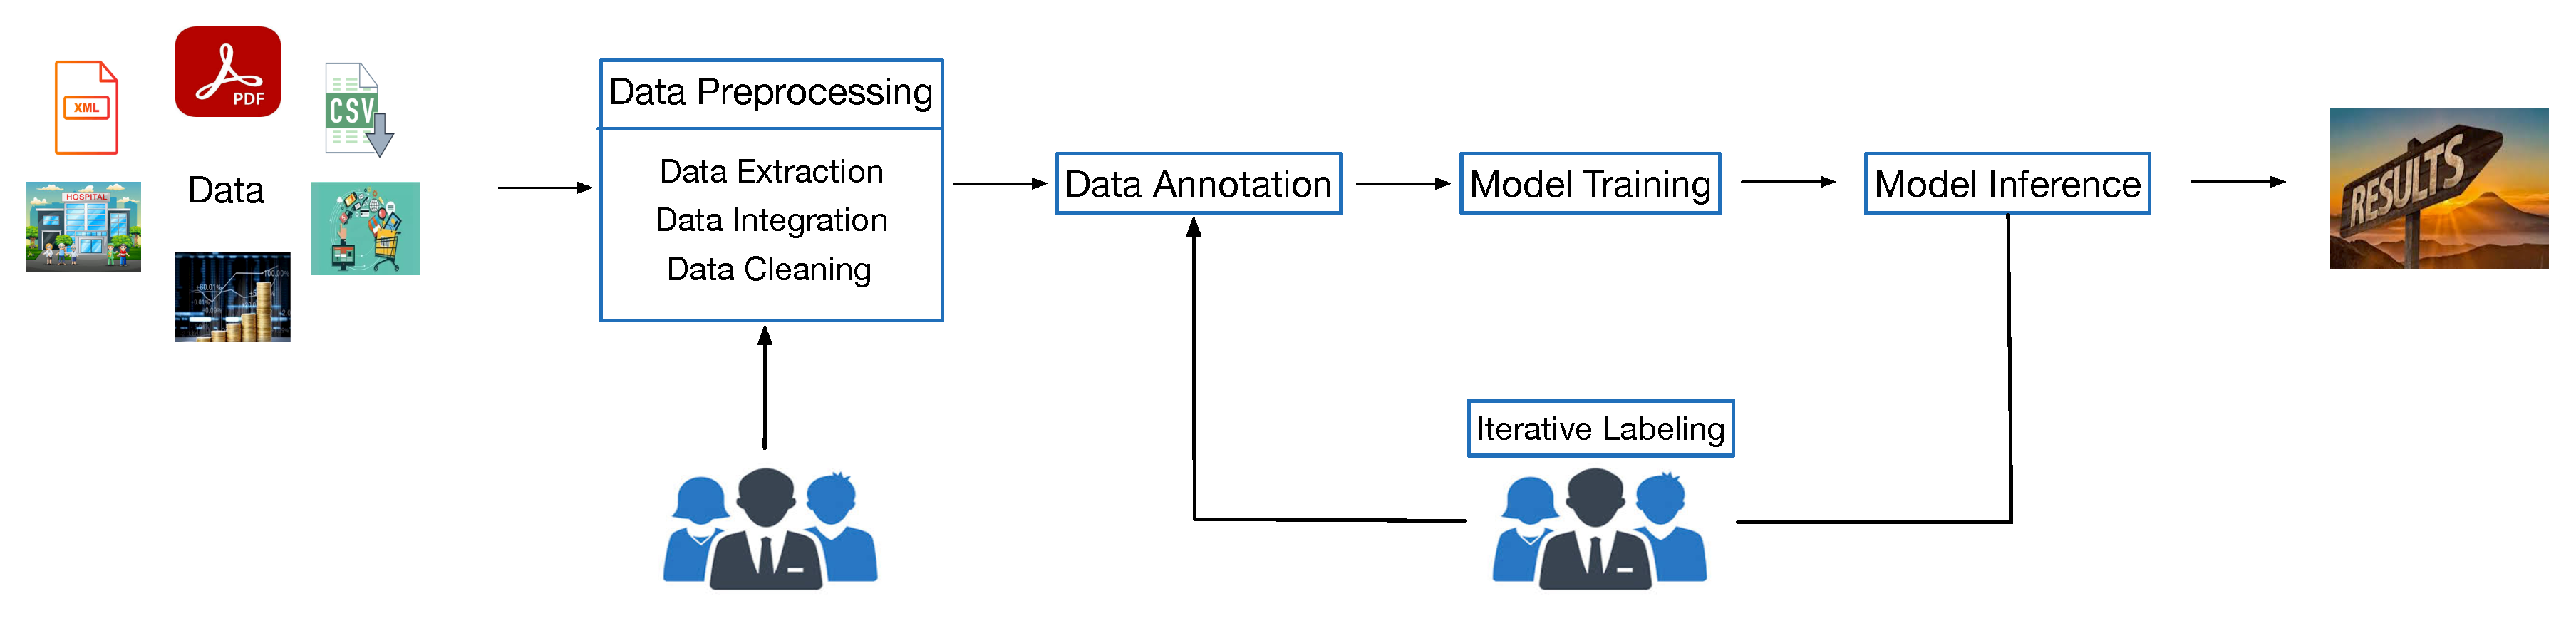
\includegraphics[width=0.65\textwidth]{
%NSFcore-2023/framework.pdf}
 %%\caption{Proposed Project}\label{project}
%\end{wrapfigure}



%We intend to propose complete, partial (either order or unordered), and various qualitative individual preference elicitation models.  An example of the first two would be having complete or only top-$k$ order of preferences over the candidates as inputs, whereas, an example of the last one  would be to bucketize candidates in different qualitative groups (recall the motivating example). For fairness, our effort would be to design group based fairness criteria designed over the protected attributes of the candidates that resemble group fairness criteria, such as, demographic parity, or statistical parity, studied in the context of classification~\cite{verma2018fairness}. To that end, we will adapt proportionate-fairness or p-fairness~\cite{pfair,chairman}  from resource allocation theory that ensures proportionate representation of every group based on a protected attribute in every position of the produced results, or its generalization~\cite{amer2009group} adapted from the social choice theory to promote affirmative action~\cite{fu2006theory} in the produced results.  
%Preference aggregation would be studied considering Kendall-Tau and Spearman's Footrule Distance functions~\cite{kemeny,diaconis1977spearman}, with the objective to minimize the sum of disagreement (Kemeny Optimization) or such, akin to existing {\em (fairness unaware) classical rank aggregation problem}~\cite{dwork2001rank,ailon2008aggregating, ailon2010aggregation}. Our goal would be to make these solutions fairness aware by investigating how to combine these two somewhat conflicting aspects in a systematic manner. For each of these proposed problem variants, we shall analyze the nature of the problem analytically and design scalable solutions with theoretical guarantees. Finally, we will perform both qualitative and quantitative study to develop actionable interventions by leveraging our proposed framework to promote fairness in two compelling applications: (i) Ranked Choice Voting (RCV)~\cite{rcv1,rcv2}, and (ii) Gender and diversity gap in the Oscars. We intend to fine-tune our proposed models based on these evaluations. 

\noindent {\bf Comparison with Existing Work.}
This contribution builds on our work recent works on fairness~\cite{islam2022satisfying, wei2022rank}, and prior works on preference aggregation~\cite{amer2009group, amer2015group, basu2015group}, studying robustness~\cite{roy2014exploiting}. We acknowledge that the existing popular group based fairness definition, such as, {\em statistical parity}~\cite{dwork2012fairness} is somewhat similar to one of our proposed fairness notion. However, the best adapted version of top-$k$ statistical parity studied in a recent paper~\cite{vldbrank} does not account for proportionate representation in every position of the top-$k$, limiting its applicability.  Studying computational challenges related to computing the margin of victory  has been a focus of recent research~\cite{stv1,stv2, stv3} in the context of electoral voting and related applications. But none of these existing works study the general version of the problem, which is, how to promote additional simple/complex constraints/criteria in the output, which is our primary focus. Other than these prior works, which are  much narrow in scope, we are unaware of any computational work that systematically studies different preference elicitation models, multiple output changing criteria, and preference aggregation combining these two.  

%Section~\ref{related} provides an in-depth comparison between our proposed work and existing work.  
%To the best of our knowledge, we are the first to investigate a generic framework that can minimally update original outcome of preference aggregation to satisfy complex constraints without any assumption on the relationship among the attributes.

%Using the aforementioned example, if $k=12$, existing work~\cite{vldbrank} only ensures p-fairness of the aggregated rank at position $12$, but not for the remaining positions (e.g., 1 to 11). {\em While p-fairness promotes stronger notion of fairness, and our proposed framework adapts to top-$k$ statistical parity, existing work does not adapt to our proposed optimization framework}.

%\smallskip \noindent {\bf Aim 1 - Fair Rank Aggregation.}
%We will begin our study in the context of ranking, which is a commonly used method to prioritize  desirable outcomes among a set of candidates and is an essential step in  many high impact applications. Here the members elicit a {\em complete preference order} over the candidates and the goal is to produce an aggregated ranked order over all candidates or produce top-$k$ results that minimize disagreements  among individual preferences. When fairness is studied, our goal would be to ensure fair representation of the candidates based on their one or more protected attributes (such as, gender, race, etc.) in the ranked order. 
%\smallskip \noindent {\bf Aim 2 - Fair Partial and Qualitative Preference Aggregation.}
%In this aim we shall consider scenarios where either qualitative preferences or partial rankings are elicited from the members. 
%We consider three such preferences: (1) top-$t$ ranking, where the input preference is a ranking of the top-$t$ items (candidates), (2) subset selection, where the input preference is an unordered subset of favorite elements, and (3) bucketing, where the input preference is a partition of the elements into three subsets: the ``yes'' set, ``ambivalent'' set, and the ``no'' set.  In our preliminary work, we consider the selection of council members or a committee of $k$ members from $n$ candidates considering the votes of $m$ judges (voters) ({\em ranked choice voting}~\cite{rank1} could be considered as a popular application of that).  The fairness criterion models affirmative action and includes a lower and upper bound on the number of elected candidates, for each value of the protected attributes(s). We intend to study the design choices of different preference elicitation models considering fairness, formalize the optimization problems and analyze them, and design principled solutions with guarantees.

%The mechanism we focus on to aggregate the top-$k$ rankings is {\em Ranked choice voting (RCV)}, and specifically RCV employing a single transferable vote (STV) system~\cite{rcvdesc}.
%We are going to follow the mechanism used in Cambridge MA to elect its city council. 

%\smallskip \noindent {\bf Aim 3 - Actionable Fair Preference Aggregation.}
%Although the proposed models and algorithms consider 
%fairness in its design, rather than an afterthought, the third aim will delve deeper into fairness considerations of compelling applications and develop actionable interventions. In particular, the third aim will provide a holistic large-scale study over two compelling applications and present actionable interventions to promote fairness. In the first application, we will study fairness in Ranked Choice Voting (RCV)\footnote{\small https://qz.com/1676718/the-pros-and-cons-of-ranked-choice-voting/} considering the data provided by the Cambridge, MA
%City Council Election 2019~\cite{RCV} to analytically answer important questions raised in recent research~\cite{rcv1,rcv2,rcv3, rcv4,rcv5}. 1. Does more choice lead to reduced racially polarized voting? 2. Does ranked choice voting enable minority representation?  Based on the analysis, {\em we will develop actionable interventions by leveraging our proposed framework to mitigate these risks}. We will perform both qualitative and quantitative analysis. For qualitative  analysis, we will recruit experienced workers from Amazon Mechanical Turk (the budget justification provided further details). A similar  study would be conducted to investigate the gender and diversity gap in the Academy of Motion Picture Arts and Sciences decisions by combining it with large scale Movielens~\cite{movielens} data and we will develop actionable recommendation to mitigate the gap. Further evaluation plan considering other datasets is described in Section~\ref{eval}.

%\section{Introduction}
\label{seC:intro}
% Interpretability and nutritional labels, generally

An essential ingredient of successful machine-assisted decision-making, particularly in high-stakes decisions, is interpretability --– allowing humans to understand, trust and, if necessary, contest, the computational process and its outcomes.   These decision-making processes are typically complex:  carried out in multiple steps, employing models with many hidden assumptions, and relying on datasets that are often repurposed --- used outside of the original context for which they were intended.\footnote{See Section 1.4 of Salganik's ``Bit by Bit''~\cite{salganik} for a discussion of data repurposing in the Digital Age, which he aptly describes as "mixing readymades with custommades.''}  In response, humans need to be able to determine the ``fitness for use'' of a given model or dataset, and to assess the methodology that was used to produce it.  

To address this need, we propose to develop interpretability and transparency tools based on the concept of a {\em nutritional label}, drawing an analogy to the food industry, where simple, standard labels convey information about the ingredients and production processes. Short of setting up a chemistry lab, the consumer would otherwise have no access to this information. Similarly, consumers of data products cannot be expected to reproduce the computational procedures just to understand fitness for their use.   Nutritional labels, in contrast, are designed to support specific decisions by the consumer rather than completeness of information.  A number of proposals for hand-designed nutritional labels for data, methods, or both have been suggested in the literature\cite{DBLP:journals/corr/abs-1803-09010,DBLP:journals/corr/abs-1805-03677,DBLP:conf/fat/MitchellWZBVHSR19}; we advocate deriving such labels automatically or semi-automatically as a side effect of the computational process itself, embodying the paradigm of {\em interpretability-by-design}. 

Interpretability means different things to different stakeholders, including individuals being affected by decisions, individuals making decisions with the help of machines, policy makers, regulators, auditors, vendors, data scientists who develop and deploy the systems, and members of the general public.  Designers of nutritional labels must therefore consider {\em what} they are explaining,  {\em to whom}, and {\em for what purpose}.  In the remainder of this section, we will briefly describe two regulatory frameworks that mandate interpretability of data collection and processing to members of the general public, auditors, and regulators,  where nutritional labels offer a compelling solution (Section~\ref{sec:intro:reg}).  We then discuss interpretability requirements in data sharing, particularly when data is altered to protect privacy or mitigate bias (Section~\ref{sec:intro:synth}).

\subsection{Regulatory Requirements for Interpretability}
\label{sec:intro:reg}

The European Union recently enacted a sweeping regulatory framework known as the General Data Protection Regulation, or the GDPR~\cite{gdpr}.  The regulation was adopted in April 2016, and became enforceable about two years later, on May 25, 2018.  The GDPR aims to protect the rights and freedoms of natural persons with regard to how their personal data is processed, moved, and exchanged (Article 1).  The GDPR is broad in scope, and applies to ``the processing of personal data wholly or partly by automated means'' (Article 2), both in the private sector and in the public sector.  Personal data is broadly construed, and refers to any information relating to an identified or identifiable natural person, called the {\em data subject} (Article 4).  

According to Article 4, lawful processing of data is predicated on the data subject's {\em informed consent}, stating whether their personal data can be used, and for what purpose (Articles 6, 7).
Further,  data subjects have {\em the right to be informed} about the collection and use of their data.~\footnote{\url{https://gdpr-info.eu/issues/right-to-be-informed/}}
Providing insight to data subjects about the collection and use of their data requires technical methods  that support interpretability.  

Regulatory frameworks that mandate interpretability are also starting to emerge in the US.  New York City was the first US municipality to pass a law (Local Law 49 of 2018)~\cite{Vacca}, requiring that a task force be put in place to survey the current use of ``automated decision systems'' (ADS) in city agencies. ADS are defined as ``computerized implementations of algorithms, including those derived from machine learning or other data processing or artificial intelligence techniques, which are used to make or assist in making decisions.''   The task force is developing recommendations for enacting algorithmic transparency by the agencies, and will propose procedures for: (i) requesting and receiving an explanation of an algorithmic decision affecting an individual (Section 3 (b) of Local Law 49); (ii) interrogating ADS for bias and discrimination against members of legally protected groups, and addressing instances in which a person is harmed based on membership in such groups (Sections 3 (c) and (d)); (iii) and assessing how ADS function and are used, and archiving the systems together with the data they use (Sections 3 (e) and (f)).

Other government entities in the US are following suit.  Vermont is convening an Artificial Intelligence Task Force to ``... make recommendations on the responsible growth of Vermont’s emerging technology markets, the use of artificial intelligence in State government, and State regulation of the artificial intelligence field.''~\cite{Vermont}.  Idaho’s legislature has passed a law that eliminates trade secret protections for algorithmic systems used in criminal justice~\cite{Idaho}.  In early April 2019, Senators Booker and Wyden introduced the Algorithmic Accountability Act of 2019 to the US Congress~\cite{BookerWydenClarke}. The Act, if passed, would use ``automated decision systems impact assessment'' to address and remedy harms caused by algorithmic systems to federally protected classes of people. The act empowers the Federal Trade Commission to issue regulations requiring larger companies to conduct impact assessments of their algorithmic systems.

The use of nutritional labels in response to these and similar regulatory requirements can benefit a variety of stakeholders.  The designer of a data-driven algorithmic method may use them to validate assumptions, check legal compliance, and tune parameters.  Government agencies may exchange labels to coordinate service delivery, for example when working to address the opioid epidemic, where  at least three sectors must coordinate: health care, criminal justice, and emergency housing, implying a global optimization problem to assign resources to patients effectively, fairly and transparently. The general public may review labels to hold agencies accountable to their commitment to equitable resource distribution. 


\subsection{Interpretability with Semi-synthetic Data}
\label{sec:intro:synth}

%Datasets are now increasingly used to train models to make decisions once made by humans.  In these automated systems, biases in the data are propagated and amplified with no human in the loop.  The bias, and the effect of the bias on the quality of decisions made, is not easily detectable due to the relative opacity of the system.  

A central issue in machine-assisted decision-making is its reliance on historical data, which often embeds results of historical discrimination, also known as {\em structural bias}.   As we have seen time and time again, models trained on data will appear to work well, but will silently and dangerously reinforce discrimination~\cite{propublicaJ,amazon_hiring,amazon_delivery}.  Worse yet, these models will legitimize the bias --- ``the computer said so.''  Nutritional labels for data and models are designed specifically to mitigate the harms implied by these scenarios, in contrast to the more general concept of ``data about data.''

Good datasets drive research: they inform new methods, focus attention on important problems, promote a culture of reproducibility, and facilitate communication across discipline boundaries.  But research-ready datasets are scarce due to the high potential for misuse. Researchers, analysts, and practitioners therefore too often find themselves compelled to use the data they have on hand rather than the data they would (or should) like to use.  For example, aggregate usage patterns of ride hailing services may overestimate demand in early-adopter (\ie wealthy) neighborhoods, creating a feedback loop that reduces service in poorer neighborhoods, which in turn reduces usage.  In this example, and in many others, there is a need to alter the input dataset to achieve specific properties in the output, while preserving all other relevant properties.  We refer to such altered datasets as \textit{semi-synthetic}.

Recent examples of methods that produce semi-synthetic data include database repair for causal fairness~\cite{DBLP:conf/sigmod/SalimiRHS19}, database augmentation for coverage enhancement~\cite{DBLP:conf/icde/AsudehJJ19}, and privacy-preserving and bias-correcting data release~\cite{DBLP:conf/ssdbm/PingSH17,DBLP:conf/vldb/RodriguezSPSH18}. A semi-synthetic datasets may be altered in different ways.  Noise may be added to it to protect privacy, or statistical bias may be removed or deliberately introduced.  When a dataset of this kind is released, its composition and the process by which it was derived must be made interpretable to a data scientist, helping determine fitness for use.  For example, datasets repaired for racial bias are unsuitable for studying discrimination mitigation methods, while datasets with bias deliberately introduced are less appropriate for research unrelated to fairness.   This gives another compelling use case for nutritional labels.

%To make our discussion more concrete, let us consider data scientists who must identify datasets appropriate for their task.  This is particularly important when semi-synthetic datasets are being released, to which noise is added to protect privacy, or statistical bias is removed or deliberately introduced.  For example, datasets repaired for racial bias are unsuitable for studying discrimination mitigation methods, while datasets with bias deliberately introduced are less appropriate for research unrelated to fairness.  



%\input{IEEE-data-engineering-IC1/preliminary}
\vspace{-0.2in}
\section{Formalism}\label{preliminary}
\vspace{-0.1in}
%The proposed work aims at developing an optimization guided computational framework that modifies an output obtained from a preference aggregation method applied on a preference elicitation model to produce a modified output that satisfies given criteria. The proposed work aims at developing this framework for a suite of preference elicitation models and preference aggregation methods.
%that satisfies with criteria that guides the need to change the original output minimally while producing a complete or top-$k$ (ordered or unordered) result aggregating individual preferences.

There are $4$ types of inputs that our proposed framework takes: (a)~a set $N$ of $n$ items, where each item has a set $\mathcal{A}$ of discrete attributes.  Each attribute $a\in \mathcal{A}$ has $\ell_a$ different values. (b)~a set of $m$ users, where the $i$-th user $u(i)$ provides her preference as $\sigma_i$. The users' preferences could be rank based, partial or full order, or non rank based. (c)~a distance function $\mathcal{F}$ (defined formally below) that measure the ``distance'' between a set of $m$ input preferences  $\sigma_1, \sigma_2,\ldots, \sigma_m$ and an output $\sigma$ with the required output form. The exact distance function depends on the underlying preference elicitation model and the required output form which may be either a complete ranking of the items or a subset of $k$ items, either ranked or not. (d)~a set $\mathcal{C}$ of output criteria/constraints. Some variants of our problem also include as input a budgetary constraint $B$.

%The proposed work aims at developing an optimization guided computational framework that suitably combines a suite of preference elicitation models with criteria that guides the need to change the original output minimally while producing a complete or top-$k$ (ordered or unordered) result aggregating individual preferences. %Next, we present some definitions that will be used throughout the proposal.  

\begin{definition}\label{def4}
\vspace{-0.1in}
{\bf Distance function $\mathcal{F}$.} Given $m$ input preferences  $\sigma_1, \sigma_2,\ldots, \sigma_m$ and an output $\sigma$ with the required output form, the function $\mathcal{F}(\sigma, \sigma_1, \sigma_2,\ldots, \sigma_m)$ is the distance of $\sigma$ from the input preferences  $\sigma_1, \sigma_2,\ldots, \sigma_m$.
In some cases the function $\mathcal{F}(\cdot)$ is an aggregation of a distance function between a single input preference and the output. Examples for such an aggregation are the sum of the pairwise distances and the maximum distance to any of the input preferences. In other cases $\mathcal{F}(\cdot)$ measures the minimum modification of the input preferences that would result in the preference aggregation method outputting the output $\sigma$. 
%$\mathcal{F}(\sigma, [\sigma_1, \sigma_2,\ldots, \sigma_m])$
\end{definition}

\vspace{-0.1in}
\begin{definition}\label{def1}
\vspace{-0.1in}
{\bf Output criteria/constraints.}  For an attribute $a\in \mathcal{A}$,  let $c(p_a)$ denote the cardinality constraints of items with value $p_a$ ($p_a$ is one of the $\ell_a$ possible values of attribute $a$). Given to the framework is a set $C$ of such cardinality constraints for each attribute value $p_a$, for every $a \in A$, $A \subset \mathcal{A}$. There are two explicit cases that we consider.
\begin{itemize}
    \item {\bf The output $\sigma$ is ordered and consists of $k\le n$ items.} 
    In this case the cardinality constraints are defined for every $\kappa \in [1..k]$ items, and for every  such $\kappa \in [1..k]$, the $\kappa$ top ranked items of output $\sigma$ have to satisfy these cardinality constraints.  
    %the $k$ top ranked items satisfy all cardinality constraints defined over $v$, i.e., it satisfies $c(p^v_{a_1}) \text{ AND } c(p^v_{a_2}) \text{ AND } \ldots \text{ AND } c(p^v_{a_A})$.  
     \item {\bf The output $\sigma$ is an unordered set of $k$ items.} In this case the cardinality constraints are defined for $k$ items and the items in the output set $\sigma$ have to satisfy these cardinality constraints. 
     \\ %$c(p_{a_1}) \text{ AND } c(p_{a_2}) \text{ AND }  \ldots \text{ AND } c(p_{a_A})$.  
\end{itemize}  
\end{definition}
\vspace{-0.1in}
\begin{definition}\label{def3}
\vspace{-0.1in}
{\bf A budgetary constraint.} A budgetary constraint $B$ is an upper bound on the distance of the output from the input preferences. 
%For a given distance function $\mathcal{F}(\cdot)$, 
The budgetary constraint implies that $\mathcal{F}(\sigma,\sigma_1,\sigma_2,\ldots,\sigma_m)\leq B$.  
\end{definition}

\vspace{-0.1in}
\begin{definition}\label{def2}
{\bf Preference Aggregation Considering Constraints.} 
We intend to study different types of problem definitions that require different algorithmic treatments.
Given either complete or partial preferences $\sigma_1,\sigma_2,\ldots,\sigma_m$ over the items in $N$, a preference aggregation method, a distance function $\mathcal{F}(\cdot)$, and a set of output criteria $\mathcal{C}$.
\vspace{-0.1in}
\begin{itemize}
    \item {\bf (Constrained optimization).} Produce an output $\sigma$ with the required form that minimizes $\mathcal{F}(\sigma,\sigma_1,\sigma_2,\ldots,\sigma_m)$ and satisfies $\mathcal{C}$.
    \vspace{-0.1in}
    \item {\bf (Optimization under budgetary constraints).} Produce an output $\sigma$ with the required form that optimizes $\mathcal{C}$,  while satisfying $\mathcal{F}(\sigma,\sigma_1,\sigma_2,\ldots,\sigma_m) \leq B$. (The objective function for optimizing $\mathcal{C}$ varies.)
    \vspace{-0.1in}
    \item {\bf (Bi-criteria optimization).} Given parameters $\alpha$ and $\beta$ produce an output $\sigma$ with the required form that satisfies both $\mathcal{F}(\sigma,\sigma_1,\ldots,\sigma_m) \le \alpha$ and $\mathcal{G}(\mathcal{C}) \le \beta$, where $\mathcal{G}$ is the objective function for optimizing $\mathcal{C}$.
\end{itemize}
\end{definition}
%The individual research aims will describe the various forms of preference elicitation from users and the details of the preference aggregation methods. We first delineate the need to change original output and the challenges that arise from there.
\vspace{-0.1in}
\subsection{Specifying Output Criteria}
We discuss orthogonal reasons where the original outputs coming out of the preference aggregation methods need to be ``massaged'' further. What unifies them is that these criteria are defined over one or more attributes of the items. Depending on how many attributes are involved in the definition and their relationship thereof gives rise to additional challenges.


%\vspace{-0.1in}
%\subsection{Important Concepts and Definitions}\label{pre}
%\vspace{-0.1in}
%\noindent \textbf{Database.} contains $n$ items or candidates. These two terms will be used interchangeably. The set of items will be denoted $V$, individual items will be denoted by $u$ and $v$. \\
%\noindent {\em \bf Individual preference Elicitation:} We consider the following individual preference elicitation models. \\
%\noindent (1) Complete preference: Each of the $4$ members (Judges) may provide a {\em complete order of preference} over the $12$ candidates (Refer to Table~\ref{tab:example_original_rank}). \\
%\noindent (2) Partial preference: 
%(2.1) Ordered. Member 1 (as well as other members) may provide a partial order over the first $5$ candidates and does not specify anything for the rest.\\
%(2.2) Unordered. Member 1 (as well as other members) may also specify that she likes the first $5$ candidates without specifying any order among them.\\
%\noindent (3) Qualitative Preference: Contrarily, Member 1 (as well as other members) may provide {\em qualitative preferences}: Molly and Amy are preferred, Abigail, Kim, Lee are acceptable, the remaining ones must not be considered. These are considered to be the inputs to the framework. Please note that 2.2 is a simplified variant of this last preference elicitation model.

%\noindent \textbf{Multiple Preferences.} The input consists $m$ different preference elicitation (based on the individual models described above). Using the motivating example, $m=4$.

\subsubsection{Fair Preference Aggregation}
We will study fairness in the context of group based protected attributes of the candidates. Output criteria/constraints for fairness (refer to Definition~\ref{def1}) are expressed over one or more {\em protected attributes}. Their protected attributes could be expressed over gender, ethnicity, race, or the state the candidates are living in. 

Formally speaking, each item/candidate $v\in N$ has one or more  {\em protected attributes}. When $\ell_a=2$, it is a binary protected attribute; when $\ell_a \geq 2$ it is a multi-valued protected attribute. As an example, race is (usually) a multi-valued protected attribute, and gender is sometimes a binary protected attribute.

%\begin{itemize}
%\item  {\bf p-fairness.} 
\smallskip \noindent \textbf{p-fairness.}
p-fairness has been studied in the context of resource allocation satisfying temporal fairness or proportionate progress~\cite{chairman, pfair}. It was introduced in the classical  {\em Chairman Assignment Problem}~\cite{baayen1964existence, chairman} that studies how to select a chairman of an union every year from a set of  $n$ states such that  that at any time the accumulated number of chairmen from each state is proportional to its weight. 

In the context of ranking, suppose that each of the $n$ ranked items has a {\em protected attribute} $a(\cdot)$ that can take any of $\ell_a$ different values. For $p_a\in [1..\ell_a]$, let $c'(p_a)$ denote the fraction of items with protected attribute value $p_a$, that is, $c'(p_a) = \frac 1n \sum_{i=1}^n \bbone_{a(i)=p_a}$. The goal is to ensure that $c'(p_a)$ fraction (rounded either up or down) of every top $\kappa$ items have protected attribute value $p_a$.
\iffalse
\vspace{-0.1in}
\item {\bf Generalization of p-fairness to promote affirmative action.} Instead of requiring $c'(p_a)$ fraction of every top $\kappa$ items to have protected attribute value $p_a$, we may want that certain values of the protected attribute get higher representation among the elements at the top, more than their overall proportion. Let $P$ be a non-negative doubly stochastic $n \cdot \ell_a$ matrix. The goal is to ensure that $P(\kappa,p_a)$ fractions (rounded either up or down) of the top $\kappa$ items to have value $p_a$, for every $\kappa \in [1..n]$ and $p_a\in [1..\ell_a]$ (if it is feasible).
It is not difficult to note that such a generalized notion can capture affirmative action.
%\end{itemize}
\fi


\subsubsection{Robust Preference Aggregation}
Output criteria/constraints for robustness on the other hand investigates the flip questions: Given either complete or partial preferences $\sigma_1,\sigma_2,\ldots,\sigma_m$ over $n$ items, let $\sigma$ be the output obtained by the preference aggregation method. Given a budget $B$, how to  make $B$ or less changes in the original preferences, such that the outcome is different from $\sigma$? This question is  related to finding the {\em margin} in electoral systems and quantifies how manipulable the underlying aggregation method is. We study this problem under different manipulation models -- addition only, deletion only, or substitution (addition + deletion).

\iffalse
\subsection{Challenges in Handling  Complex Output  Criteria}
In general, the output requirements/constraints are defined over a set $R$ of attributes. When $|R|=1$, as an example, the output requirement is defined on a single attribute (such as race). In a recent work, we demonstrated that for an aggregation method that models plurality voting, the problem of preference aggregation while satisfying output criteria defined by a single attribute is computationally easy. 
However, the nature of the problem changes when two or more attributes are involved in the output criteria. In Section~\ref{aim1} we discuss this more complicated case and refer to our recent work in which we showed evidence that in some cases it is computationally difficult even to find any output with the required form. 
\fi
%When there are two or more different attributes involved in outlining output criteria/constraints (such as certain representation from race and certain representation from gender), the PIs have proved in a recent work~\cite{islam2022satisfying} that the decision version of the preference aggregation problem under output constraint becomes (weakly) NP-hard by reducing the well known NP-hard Partition problem to our problem~\cite{garey1979computers}. We note that the existing practice of converting multiple attributes to a single multi-valued protected attribute by computing joint distribution over the attributes assumes independence among the attributes. When Independence among the attributes does not hold, this simplification leads to a heuristic process.  The PIs have also demonstrated that for three (or more) attributes (e.g., constraints defined over race, and gender, and ethnicity), even the question whether there exists a set of top-$k$ that satisfies the complex constraint is strongly NP-Hard where the reduction is fro 3 Dimensional Matching. On the positive side for the case of two  attributes, the PIs have designed an efficient algorithm a preference aggregation algorithm while satisfying fairness constraints defined over $2$ attributes and has designed a 2 approximation factor and runs in $O(n^2\ell \log m)$ time, by casting this problem as a min cost flow problem, where $\ell$ is the total number of possible attribute values. We intend to study these aspects in the proposal - as it turns out to be an intellectually demanding and independent  facet of the computational problem, irrespective of the specific reasons to change the output.


%\input{IEEE-data-engineering-IC1/aim1}
\vspace{-0.2in}
\section{Single Round Rank based Preference Aggregation}\label{aim1}
\vspace{-0.1in}
We outline two separate lines of algorithmic problems: (1) incorporating output criteria (e.g., p-fairness) in single round rank-based preference aggregation methods, and (2) satisfying complex constraints in single round rank-based preference aggregation methods.
\vspace{-0.1in}
\subsection{Incorporating output criteria in rank aggregation} 
\vspace{-0.1in}
The input to the classical {\em rank aggregation} problem consists of $m$ complete order of preferences over the $n$ items/candidates. Traditionally, producing the final ranking involves aggregating potentially conflicting preferences from multiple individuals, and is known as the rank aggregation problem~\cite{dwork2001rank,van2007deterministic, ailon2008aggregating}. Our goal is to  minimally change the aggregated output to enable fairness.
%p-fairness has been studied in the theory community to enable resource allocation satisfying temporal fairness or proportionate progress.
We will study p-fairness~\cite{chairman, pfair} that ensures proportionate representation of every group based on a protected attribute in every position of the aggregated ranked order.  The classical problem in this context is known as the {\em Chairman Assignment Problem}~\cite{baayen1964existence, chairman} which studies how to select a chairman of a union every year from a set of  $r$ states such that  that at any time the accumulated number of chairmen from each state is proportional to its weight. p-fairness generalizes other notions of fairness~\cite{islam2023equitable} that were considered in prior work, including the existing popular group based fairness definition {\em statistical parity}~\cite{dwork2012fairness}. 
%We start with some definitions and then describe both our preliminary research and the open problems we plan to investigate further.
\vspace{-0.1in}
\subsubsection{Research Directions}
\vspace{-0.1in}
%\noindent \textbf{Rank and Multiple Ranking.}  
Consider rankings of the items in a set $V$. Each such ranking can be viewed as a permutation. We will use the terms ranking and permutation interchangeably. 

\noindent \textbf{Kendall-Tau and Kemeny distances.}
	Given two rankings $\sigma,\eta: V \rightarrow [1..n]$, the
	Kendall-Tau distance between the two rankings is the sum of pairwise disagreements between $\sigma$ and $\eta$ (bubble-sort distance)
	\[
	\cK (\sigma,\eta) = \sum_{\{u,v\}\subseteq V} \bbone_{(\sigma(v)-\sigma(u))(\eta(v)-\eta(u))<0}.
	\]
	
	For a set of rankings
	$\{\eta_1,\eta_2,\ldots,\eta_m\}$ the {\em Kemeny distance} of the ranking
	$\sigma$ to this set as
	\[
	\kappa(\sigma,\eta_1,\eta_2,\ldots,\eta_m)= \sum_{i=1}^m \cK (\sigma,\eta_i).
	\]

 \noindent \textbf{Spearman's footrule distance.}
    Given two rankings $\sigma,\eta: V \rightarrow [1..n]$, the 	Spearman's footrule distance between the two rankings is the sum of the absolute values
  ($\ell_1$ distance) of the differences between rankings $\sigma$ and $\eta$.
	\[
	\cS (\sigma,\eta) = \sum_{u\in V} |(\sigma(u)-\eta(u)|
	\]
 
	For a set of rankings
	$\{\eta_1,\eta_2,\ldots,\eta_m\}$ the {\em Spearman's footrule distance} of the ranking
	$\sigma$ to this set is the sum of the pairwise distances.

    \noindent \textbf{Rank aggregation.} The aggregated ranking of a set of $m$ rankings $\{\rho_1,\rho_2,\ldots,\rho_m\}$ for a given distance function is a ranking that minimizes  the distance to this set.
    
    \noindent \textbf{p-fairness for a ranking.}
    For a permutation $\sigma, k\in [1..n], p\in [1..\ell]$, let $P(\sigma,k,p)$ denote
    the number of elements with protected attribute value $p$ among the $k$ top ranked elements
    in $\sigma$. A ranking $\sigma$ is {\em proportionate fair} or {\em p-fair} if
    \[
    \forall k\in [1..n]\, \forall p\in [1..\ell]:\  P(\sigma,k,p)\in \{\floor{f(p)\cdot k},\ceil{f(p)\cdot k}\}.
    \]

 
%We note that the best adapted version of top-$k$ statistical parity studied in a recent paper~\cite{vldbrank} does not account for proportionate representation in every position in the top-$k$ positions, but just to a small number of positions, thus limiting its applicability.
%As a matter of fact it can be shown that the algorithm Fair-ILP presented in~\cite{vldbrank} for the special case of a binary protected attribute in which the frequency of both values is the same may produce a very skewed output. This is because the algorithm Fair-ILP just considers the {\em total number of times} items with one value of protected attribute are ranked above items with the other value. p-fairness is  stronger because it ensures statistical parity for every position in the ranked order and considers, for every $k$, the number of times items in the top-$k$ with one value of protected attribute are ranked above items with the other value. This makes this notion of fairness significantly harder to implement and the existing solutions do not trivially adapt.


We formalized two optimization problems, individual p-fairness or {\bf IPF} and the rank aggregation problem subject to proportionate fairness ({\bf RAPF})  considering binary ($\ell=2$) and multi-valued ($\ell > 2$) protected attributes. These problems and associated algorithmic results could be found in~\cite{wei2022rank}.


\vspace{-0.1in}
\subsubsection{Open Problems}
\vspace{-0.1in}
We plan to investigate the following open problems.

\smallskip \noindent{\bf p-fairest aggregate ranking (PFAR).} 
The PFAR problem is defined as follows. Given a set of $m$ rankings %$\{\rho_1,\rho_2,\ldots,\rho_m\}$ 
choose the ``p-fairest'' ranking among all rankings that minimize the Kemeny distance to this set. 
We need to define ``p-fairest'' ranking or a distance measure to a p-fair ranking.
We propose the following distance measure (using the notations defined above).
For an integer $d \ge 0$, a ranking $\sigma$ is at distance $d$ from a {\em p-fair} ranking if
\[
\forall k\in [1..n]\, \forall p\in [1..\ell]:\  P(\sigma,k,p)\in \{\floor{f(p)\cdot k}-d,\ceil{f(p)\cdot k}+d\}.
\]

\iffalse
Another way to view the distance to a p-fair ranking is by considering the classical {\em p-processor cup game} defined by Liu~\cite{liu1969} that considered the notion of p-fairness in multi processor scheduling. The p-processor cup game (adapted to our case) is a multi-round game with two players, an {\em emptier} and a {\em filler}, that takes place on $\ell$ cups, each filled initially with a fixed amount of water, called {\em buffer}. At the beginning of each round,
the filler adds a total of 1 gallon of water to the cups. The distribution of this 1 gallon to the cups is determined by the filler.
The emptier then selects a single cup (that must have at least 1 gallon of water)
and removes 1 gallon from this cup. The emptier’s goal is to minimize the size of the buffer and the {\em backlog} which is the amount of water (on top of the initial amount) in the fullest cup.

It is easy to see the analogy to p-fairness. Consider a p-fair ranking of $n$ elements each with a protected attribute with $\ell$ possible values. Each cup represents a possible value of the protected attribute. The corresponding game has $n$ rounds. In each round $k\in [1..n]$ the filler
adds $f(p)$ gallons of water to cup $p$, for $p\in [1..\ell]$, and the emptier removes 1 gallon of water from the cup corresponding to the value of the protected attribute of the element ranked $k$.
The existence of a p-fair ranking implies that the emptier can always guarantee that the size of the buffer and the backlog is no more than 1 gallon.
For a ranking that is at distance $d$ from a p-fair ranking, the emptier can guarantee that the size of the buffer and the backlog is no more than $1+d$ gallons.
\fi

We observe that PFAR is also NP-Hard as directly follows from the fact that unconstrained rank aggregation is NP-hard when 
$m\ge 4$~\cite{ailon2008aggregating}. For some fixed $\alpha > 1$, We would like to find an algorithm that finds the p-fairest ranking among all rankings whose Kemeny distance from the set of input rankings is at most $\alpha$ times the minimum such distance. 
%Reasonable values of $\alpha$ to consider are 
%$\frac 85$ and $\frac 43$ since there are efficient $\frac 85$ and $\frac 43$ approximation algorithm for the rank aggregation problem~\cite{ailon2008aggregating}.

\smallskip \noindent {\bf Bi-criteria p-fair rank aggregation (BPFRA).} 
The most general problem that we plan to consider in this context is the bi-criteria optimization problem, that is, for a given pair $(\alpha>1 ,\beta>1)$ and a set of $m$ rankings %$\{\rho_1,\rho_2,\ldots,\rho_m\}$
find a ranking whose Kemeny distance to the set of rankings is at most $\alpha$ times the Kemeny distance of the aggregated rank from the set and its distance from a p-fair ranking is at most $\beta$, if such a ranking exists.

\smallskip \noindent{\bf p-fair rank aggregation with affirmative action.} 
We plan to consider a variant of p-fair rank aggregation that involves ``affirmative action''. This will be modeled by varying the proportion of the values of the protected attribute in the p-fair aggregated rank. For example, consider a binary protected attribute with values A and B each needs to appear the same number of times. Suppose that our goal is to promote the items with attribute value A. In this case we can vary the proportion of A making it higher in the top ranked elements and lower in the lower ranked elements so that overall items with attribute value A will appear the same number of times as items with attribute value B.

\smallskip \noindent{\bf The complexity of individual p-fair ranking (IPF).}  We plan to further investigate the IPF problem for multi valued protected attributes as it is open whether it can be solved accurately in polynomial time. We conjecture that this problem is NP-Hard. %and plan to look for a suitable reduction to prove this conjecture. 
We also plan to look for improved approximation algorithms for this problem.
%We note that the algorithm DetConstSort given in~\cite{kddrank} does not produce closest ranking to a given input ranking.

\smallskip \noindent {\bf Better approximation of rank aggregation subject to p-fairness (RAPF).}
We plan to develop more sophisticated RAPF algorithms with better approximation ratios,  %One approach for designing such algorithms is to apply the pivoting technique presented in~\cite{ailon2008aggregating} for rank aggregation. We also plan 
and to improve the computational aspects of the RAPF problem. This problem can be formulated as an Integer Programming (IP) problem. %and thus the RAPF problem of reasonable size can be solved in practice using an IP solver like Gurobi or CPLEX.
We plan to consider various IP formulations as well as various rounding techniques to accelerate the computation.

\smallskip \noindent{\bf Robust rank aggregation.} It is known that rank aggregation under Kemeny distance is NP-hard. We will explore other aggregation methods, such as Spearman's footrule and Borda, and study how manipulable these rank aggregation methods are -- that is, if only $x\%$ of the preferences are allowed to be changed, how easy it is to change the outcome.
\vspace{-0.1in}
\subsection{Complex Constraints} 
\vspace{-0.1in}
Our goal is to optimize preference substitution to satisfy complex top-$k$ fairness constraints, where the fairness requirement is defined over a set $R$ of protected attributes. One of the objectives we will consider is {\em minimizing the number of single ballot (ranking) substitutions that guarantee fairness in the top-$k$ results.} 
%In voting theory~\cite{cary2011estimating}, the concept of margin of victory (MOV) is designed to measure electoral competitiveness of the candidates. 
In a preliminary work we defined the problem of finding the smallest number of single ballot substitutions to promote a set of $k$ candidates that satisfy fairness requirements defined over a set $R$ of protected attributes to the top-$k$. 
\vspace{-0.1in}
\subsubsection{Research Directions}
\vspace{-0.1in}
We assume that there are $\ell$ protected attributes , denoted $A_1,\dots, A_\ell$. For $i\in [1..\ell]$, attribute $A_i$ has $\ell_i$ possible values, denoted $A[i,j]$, for $j\in [1..\ell_i]$. Each candidate is associated with a specific value from each attribute.
In addition, we are given target quantities $a[i,j]$, for $i\in [1..\ell]$, and  $j\in [1..\ell_i]$, with property that all row marginals sum to $k$. Namely, for every $i\in [1..\ell]$, $\sum_{j=1}^{\ell_i} a[i,j] = k$. A fair outcome should satisfy the fairness  condition that for $i\in [1..\ell]$, and  $j\in [1..\ell_i]$, exactly $a[i,j]$ candidates whose $A_i$ attribute value is $A[i,j]$ are elected. 

\noindent We note that one way to approach this problem is by converting the multiple protected attributes to a single multi-valued protected attribute by computing joint distribution over the attributes assuming their independence. For example, instead of considering two binary valued attributes $A_1$ and $A_2$ we consider a single attribute with 4 possible values and the requirement that the value $i*j$ should appear $a[1,i]\cdot a[2,j]/k$ times, for $i,j\in \{1,2\}$. The shortcomings of this approach are two-fold: First, this approach may yield that the problem is infeasible while there is still a solution without assuming independence. A solution that assumes independence may be inferior (require more substitutions) than a solution that does not assume independence.

\noindent In~\cite{islam2022satisfying}, we showed that the problem of finding the smallest number of single ballot substitutions (original preference) to promote a set of $k$ candidates that satisfy proportionate representation over a single protected attribute is computationally easy for any domain size of the protected attribute. On the other hand the same problem becomes computationally hard if we increase the number of protected attributes. When there are two different protected attributes involved in outlining the fairness requirement, we proved that the decision version of that problem is (weakly) NP-hard, %by reducing the well known NP-hard Partition problem to our problem~\cite{garey1979computers}. 
For three (or more) protected attribute, even the question whether there exists a set of top-$k$ that satisfies the complex fairness constraint is strongly NP-Hard by a reduction from 3 Dimensional Matching. On the positive side for the case of two protected attributes we designed an efficient algorithm that obtains a 2 approximation factor and runs in $O(n^2\ell \log m)$ time, 
%by casting this problem as a min cost flow problem, 
where $\ell$ is the number of possible attribute values. We also designed an exact algorithm with running time $n^c$, where $c$ is the size of the Cartesian product of all the attribute domains.

\vspace{-0.1in}
\subsubsection{Open Problems}
\vspace{-0.1in}
There propose two possible ways to extend these problems.

\smallskip \noindent {\bf Improved approximation ratio in the case of 2 protected attributes.} 
Since  the problem of minimizing the number of single ballot substitutions in the case of 2 attributes is currently proven to be weakly NP-Hard, it may admit a PTAS (Polynomial Time Approximation Scheme). We plan to investigate the existence of a better approximation algorithm. Alternatively, we will try to improve the hardness result and show that this problem is strongly NP-Hard or Max-SNP Complete. 

\smallskip \noindent {\bf Relaxed solutions in the case of 3 or more protected attributes.} 
Clearly, the hardness result of even checking the existence of a solution in case of 3 or more attributes precludes the existence of any approximation algorithm for this case. We plan to design an algorithm that will generate a relaxed set of items/candidates. The relaxation may be in two dimensions: (i) the generated set will be a top-$k$ set of candidates but the fairness requirements will not be fully satisfied for all protected attributes. (ii) the generated set will have size larger than $k$ but it will satisfy the (lower bounds of the) fairness constraints for top $k$. Clearly, the larger the generated set is the easier the problem. We will find the smallest such extended set that guarantees the fairness  constraints imposed by all protected attributes.


%\input{IEEE-data-engineering-IC1/Aim2}
\vspace{-0.1in}
\section{Multi Round Rank based Preference Aggregation}\label{aim2}
\vspace{-0.1in}
We study algorithmic challenges to satisfy  output constraints in multi-round rank based preference aggregation methods, popularly known as ranked choice voting or (RCV)~\cite{irv1}. 
\vspace{-0.1in}
\subsection{Research Directions}
\vspace{-0.1in}
We start by describing the STV (single transferable vote) method~\cite{stv-irv, stv1} that generalizes the IRV method, and selects a set of $k$ items/candidates as the winners. STV is gaining popularity as an electoral system. It is used to elect candidates to the Australian Senate, in all elections in Malta, in most elections in the Republic of Ireland, and in Cambridge, MA. There are also plans to use STV in other USA localities. As mentioned in Section~\ref{preliminary} this method of preference aggregation is also applicable in other settings.

The input to an STV preference aggregation method consists of $m$ either complete or partial rankings of the items/candidates. Suppose that the total number of items/candidates is $n$ out of which $k$ items need to be elected. The preference aggregation process requires a predefined {\em quota}. In most cases this quota is Droop quota~\cite{droop} defined as $\floor{\frac{n}{k+1}}+1$. The aggregation is done in rounds. In each round every item/candidate is associated a {\em tally}. Initially, the tally of every item is the number of rankings in which it is ranked highest. A round starts by considering the items whose tally is at least the quota. These items are elected in non-increasing order of their tally, as long as $k$ items/candidates have not been elected (which always holds for Droop quota). When an item is elected their ``surplus'' (the number by which their tally exceeds the quota) is distributed to the next preferred item in their ranking (that has not been eliminated yet). The exact way this ``surplus'' is allocated varies. In a most cases, this allocation is done either fractionally or by a random selection of the surplus rankings out of all the  rankings in which the elected item is top ranked. This is repeated as long as there are items whose tally is at least the quota (and $k$ items/candidates have not been elected). 
Then, if less than $k$ items/candidates are elected, the item/candidate with the smallest tally is eliminated from all the rankings, and the tallies are updated based on the new rankings. If the number of items/candidates remaining (not elected and not yet eliminated) equals the
number of items/candidates left to be elected, these candidates are elected and the STV process terminates, otherwise the process repeats.

There is evidence that IRV and thus also STV preference aggregation methods are computationally hard to manipulate. It is NP-Hard to decide whether an IRV method can be manipulated even by adding one complete ranking~\cite{stv2}. On the positive side, \cite{blom2016,blom2019,magrino2011} suggested branch and bound algorithms that use Integer Programming to compute the Margin of Victory (MOV) in IRV. 

\iffalse
In our preliminary work, 
we considered the selection of $k$ council members out of $n$ {\em candidates} by $m$ voters or {\em members} with no ranking among the $k$ selected candidates. The fairness criterion %for this scenario is quite straightforward: 
is to maintain the proportion of each value of the protected attributes(s) within the selected candidates as in the whole set of candidates, or its generalization that models affirmative action and includes a lower and upper bound on the number of elected candidates, for each value of the protected attributes(s). %Since sometimes affirmative action is required, we consider a generalization where for each value of the protected attributes(s) we are given a lower and upper bound on the number of candidates with this value who have to be elected to the committee.
The challenge is how to produce a fair (or close to fair) solution that accurately reflects the opinions of the voters.

One obvious way is to elicit preference from the members is to ask each member or voter to vote for (up to) a fixed number $t \in [1..k]$ candidates and choose the $k$ candidates who received the most votes, and satisfy the fairness constraints. A clear shortcoming of this simplistic approach is that some of the elected candidates may receive very little support by the voters. For example, in case each voter casts a vote for a single candidate and one of the candidates is endorsed by, say, $90\%$ of the voters, then the rest of the elected candidates would each be elected by less than $10\%$ of the voters. 

Another option is to ask the voters to rank the candidates and then use p-fair rank aggregation as discussed earlier to identify the top $k$ candidates. This option is also not desirable. First, it requires the voters to rank all candidates. Second, this method has some inherent shortcomings as per the celebrated Arrow's impossibility theorem~\cite{arrow,fishburn1970arrow}. These shortcomings are apparent in the specific rank aggregation method used earlier, as this method satisfies the {\em extended Condorcet criterion}, and thus may give total power to a slim majority, ignoring the opinion of a sizable minority. For example, consider the case of $100$ voters and $26$ candidates among whom 13 candidates need to be elected.
Denote the candidates by the letters $A,\ldots,Z$. Suppose that 51 of the voters rank the candidates in order from $A$ to $Z$ while 49 of the voters rank the candidates in reverse order from $Z$ to $A$. The aggregated rank will be $A,\ldots,Z$, implying that the 13 elected candidates will be $A,\ldots, M$, and none of the candidates preferred by 49 of the voters will be elected.

An alternative option that we explore and is regaining popularity recently is the {\em ranked choice voting (RCV)}~\cite{rank1}, and specifically RCV employing a {\em single transferable vote (STV)} system. An STV-RCV means an electoral system in which voters rank up to a fixed $t \in [1..k]$ candidates and ballots transfer to next‐ranked picks until all seats are filled. Broadly, such systems can facilitate majority winners in single‐seat elections, and majority rule with minority representation in multi‐seat elections. There are numerous mechanisms to determine the winners in an STV-RCV. We follow the mechanism used in Cambridge MA to elect its city council as described below (source~\cite{rcvdesc}).

Once ranked ballots have been collected, winners are determined in rounds that are repeated as long as there are still seats that need to be filled.
Each round is called a {\em count}. 
A {\em quota} is set to $q=\floor{n/(k+1)}+1$. %$q=\floor{\frac{n}{k+1}}+1$.
The process in each count is as follows. 
\begin{itemize}
    \item
    If the number of candidates remaining equals the number of seats left to be filled, then all remaining candidates are elected.
    \item 
    Else if the number of first-place votes for a specific candidate is at least the quota $q$, then this candidate is
    elected. The ``surplus'' first-place votes for this candidate, i.e., all votes over $q$ votes, are
    randomly\footnote{The selection is not actually random in the mechanism used in Cambridge MA}
    selected to be transferred to the next candidate(s), as explained below.
    This process is repeated for all candidates who got at least $q$ first-place votes.
    \item
    Otherwise, the candidate with the least first-place votes is eliminated. All the  of first-place votes for the eliminated candidate are transferred, as explained below.
\end{itemize}

The transfer of votes is done by simply erasing the first-place votes in all ballots in which votes need to be transferred,
and treating the second-place vote as the new first-place (if the second-place candidate has been elected or eliminated already, then the votes are transferred further).

This STV-RCV mechanism has the property that minority votes are reflected in the results. As a matter of fact it is shown in~\cite{rcv4} that if for some integer $k>0$ a coalition of at least $k\cdot q$ voters prefers $k$ candidates over the other candidates, then these candidates are guaranteed to be elected. 
\vspace{-0.1in}
\subsection{Open Problems}
\vspace{-0.1in}
\smallskip \noindent {\bf Fair STV-RCV.}
The goal is to develop a fairness aware STV-RCV, using the fairness criterion defined above that still maintains an adequate representation to coalitions. 

We note that the mechanism described above can be modified to satisfy fairness as follows. %First, define some notations.
For $p\in [1..\ell]$, let $\textsc{Cand}(p)$ be the set of all candidates whose protected attribute has value $p$, and let $Upper(p)$, and $Lower(p)$ be the upper and lower bounds on the number of elected candidates from $\textsc{Cand}(p)$ as dictated by the fairness requirement.
To achieve the fairness criterion each count needs to follow the following rules: 
(i) Whenever the number of currently elected candidates from $\textsc{Cand}(p)$ reaches $Upper(p)$, all the votes for other candidates in $\textsc{Cand}(p)$ are transferred. (ii) For any $p\in [1..\ell]$, if the number of currently elected and remaining candidates from $\textsc{Cand}(p)$ equals $Lower(p)$,
then all the remaining candidates from $\textsc{Cand}(p)$ are elected. 
(iii) Let $P\subseteq [1..\ell]$ be the set of all values $p\in [1..\ell]$ for which the number of currently elected candidates from $\textsc{Cand}(p)$ is strictly less than $Lower(p)$, and let $\bar{P}$ be the complement set. Define $S$ to be the sum the differences between $Lower(p)$ and the number of currently elected candidates from $\textsc{Cand}(p)$, for all values of $p\in P$. If $k$ minus the total number of currently elected candidates equals $S$, then the votes for all the remaining candidates in $\cup_{p\in \bar{P}} \textsc{Cand}(p)$ are transferred. 

Clearly, the coalition property of STV-RCV is not maintained in the fairness aware mechanism. We plan to investigate the trade-off between fairness and the power of coalitions and come up with bi-criteria optimized mechanisms.   

\smallskip \noindent {\bf Fair Unordered Partial Preference Aggregation.}
Next, we consider a scenario where partial rankings are elicited from the members (voters). Specifically, each voter specifies a subset of cardinality at most $t$ of elected candidates. Recall that the classical rank aggregation algorithms  are generalized to handle also ties (see, e.g.~\cite{fagin2004comparing}). 
We view each individual preference as a ranking with ties, where
all candidates in the selected subset are tied and above the candidates not in the subset which are also tied. 
We note that in this case the rank aggregation with ties algorithms will not give power to a slim majority as was the case for a complete order. Consider the scenario defined above of $100$ voters and $26$ candidates, $A,\ldots,Z$, among whom 13 candidates need to be elected.
Assume that 51 of the voters elect the subset $A,\ldots,M$ while 49 of the voters elect the complement subset $N,\ldots,Z$. The aggregated rank will be have 7 candidate from $A,\ldots,M$ and 6 from $N,\ldots,Z$. Thus, giving representation also to the minority.  

%\noindent {\bf Problem 2.2: Design a fairness aware mechanism for subset election.}
It can be shown that computing rank aggregation with ties subject to the fairness constraints defined above is NP-hard by reduction from MAX2SAT problem. Thus we plan to consider the problem of finding an efficient approximation algorithm for this problem. We also plan to consider the bi criteria version of this problem where we allow to relax the fairness constraints if it results in a better rank aggregation.

\smallskip \noindent {\bf Fair  Qualitative Preference Aggregation.}
The third scenario we consider is bucketing, in which each individual preference is a partition of the elements into three subsets: set $Y$ of the liked candidates,
set $A$ of the candidates for which there is no firm preference, and set $N$ of the disliked candidates. One obvious way to handle this case is again to consider it as an instance of rank aggregation with ties where we have all the candidates in $Y$ ranked above the candidates in $A\cup N$, and all the candidates in $A$ ranked above the candidates in $N$. The weakness of this approach is that it does not distinguish sometimes between the disliked candidates and the candidates with no firm preference. Specifically, the case of having $k$ candidates liked by a slim majority of the voters but disliked by the rest would be treated the same way as the case of having $k$ candidates liked by a slim majority of the voters and no firm preference by the rest.
Motivated by this example we propose to consider the {\em controversy} of a candidate $c$ and define it as the number of pairs of voters that have contradicting preference of $c$, i.e., the number of pairs of voters for which $c \in Y$ for one voter and $c\in N$ for the other. We intend to study this variant as an open problem.
\fi 

\smallskip \noindent {\bf Approximating the number of ranking substitutions in multi round methods.} 
We plan to develop approximation algorithms with proven performance for IRV and STV. The first step is to design such an algorithm for the simplest case which is approximating the minimum number of ranking substitutions required to change the outcome of an IRV preference aggregation method when every user is limited to input only two top items. From there we hope to be able to generalize to the IRV problem with no restriction on the ranking size, and eventually to the more general STV.

\smallskip \noindent {\bf Improved computational frameworks for minimizing number of ranking substitutions in multi round methods.} 
As mentioned above most of the existing computational frameworks are based on branch and bound algorithms. We plan to investigate other methods and possibly alternative formulation of the respective Integer Programming model that may result in more efficient computational frameworks.

\smallskip \noindent {\bf Heuristic algorithms for minimizing the number of ranking substitutions in multi round methods.} 
Another way to tackle the complex computational problem of minimizing number of ranking substitutions in multi round methods is designing heuristics for this task, analyzing and benchmarking these heuristics. One approach for designing such a heuristic for the problem of minimizing the number of ranking substitutions in STV to guarantee an elected set of $k$ items with a given requirement on their protected attribute is by first identifying the desired elected set and then computing the number of substitutions required to achieve this set. One way of fixing the desired set is as follows. Run the STV process, and whenever the number of the currently elected items/candidates with a given value of their protected attribute reaches its bound, eliminate all the items/candidates with this value of their protected attribute. A naive implementation of this rule may not even guarantee a feasible solution and thus we also need to add the option of reintroducing items/candidates that were already eliminated. Analyzing such an algorithm is a challenge.



%\input{IEEE-data-engineering-IC1/nonrank}
\vspace{-0.1in}
\section{Non-rank based Preference Aggregation}\label{nonrank}
\vspace{-0.1in}
Our goal is to study preference  models that allow users to elicit their choice not as a ranked order. When the input preferences are not ranked, the output produces a set of $k$ items that best reflects the users preferences. Akin to the previous two sections, our goal is to investigate which preference aggregation methods are suitable for such elicitation models, how to handle output constraints, and understand their computational implications. We identify the following research directions.
\vspace{-0.1in}
\subsection{Research Directions}
\vspace{-0.1in}
We begin by considering simple Boolean preference elicitation models, as``only likes'', ``likes and dislikes'' , or ``only dislikes''. Indeed, such preference elicitation models are realistic in a wide variety of applications, such as providing preferences over products, news articles, movies, songs, social media posts, to name a few.

The simplest form of preference elicitation comes in the following form - each user $u(i)$ provides $\sigma_i$ as preference, which is a Boolean vector of $1$'s and $0$'s over the set of $n$ items, and the underlying application \textit{only objective} is to find a set of $k$-items that are ``most liked'' by all the users. We propose to use Jaccard similarity or overlap similarity~\cite{roy2014exploiting} for measuring similarity (inverse of distance) between two vectors in such cases. Given two vectors $\sigma_i, \sigma_j$ their overlap similarity $S_{\sigma_i, \sigma_j} = \sum_{\forall \ell \in [n]} [\sigma_{i_\ell} \land \sigma_{j_\ell}]$, the number
of positive bits that are shared between $\sigma_i, \sigma_j$. When  the users provide both ``likes'' and ``dislikes'' and both have to be accounted for, we will use Hamming Distance  which measures the minimum number of substitutions required to change $\sigma_i$ to  $\sigma_j$. 

We have explored two alternative preference aggregation methods~\cite{amer2009group, roy2014exploiting} in the past that serve as the basis of this study.
\begin{itemize}
    \item \textbf{Aggregated Voting.} Produce $\sigma$, such that $\mathcal{F}(\sigma,\sigma_1) + \mathcal{F}(\sigma,\sigma_2) +\ldots \mathcal{F}(\sigma,\sigma_m)$ is minimized.
     \item \textbf{Least Misery.} Produce $\sigma$, such that $\mathbf{Maximum}\{\mathcal{F}(\sigma,\sigma_1), \mathcal{F}(\sigma,\sigma_2),\ldots \mathcal{F}(\sigma,\sigma_m)\}$ is minimized.
\end{itemize}
The goal is to produce $\sigma$, which is also a vector of length $n$ with exactly $k$ number of 1's and remaining $0's$ that minimizes the Inverse of overlap similarity/Hamming Distance, denoted $\mathcal{F}(\cdot,\cdot)$, between $\sigma$ and $\{\sigma_1,\sigma_2,....\ldots,\sigma_m\}$.

We realize that the overlap similarity function is monotone, as when a new item is considered in the mix, the overlap similarity can never decrease (or inverse overlap similarity can never increase). This is likely to make preference aggregation computationally tractable and give rise to polynomial time solution to produce optimal $\sigma$. Under Hamming distance, however, finding $\sigma$ considering either of the preference aggregation models is likely to be NP-hard, as a known NP-Complete problem Median String Problem could be reduced to a variant of this problem~\cite{de2000topology}. \\
{\bf Satisfying Output Constraints.}
The output constraints in this case are defined on the top-$k$ items/candidates and involve one or more protected attributes. When the output criteria is simple (designed on a single attribute),  the Preference Aggregation Problems Considering Constraints  defined in Section~\ref{preliminary} for aggregated voting under Overlap Similarity is likely to give rise to computationally tractable problem for all three variants - Constrained optimization, Optimization under budgetary constraints, and Bi-criteria optimization. On the other hand, these problems are likely to be computationally harder for least misery under Overlap Similarity. We will study how to exploit the monotonicity property of overlap similarity to see if it is possible to design greedy algorithms with provable approximation factors. Under Hamming Distance, irrespective of the underlying aggregation method, the Preference Aggregation Problems Considering Constraints are likely to be NP-hard, since the Preference Aggregation under Hamming Distance itself is NP-hard. We intend to study the possibility of designing approximation algorithms as well as efficient heuristics for these problems.
\subsection{Open Problems}
The applicability of the ordinal preference model is explored as one of the open problems - an ordinal value $g$ is defined on an $s$-point performance scale, that is totally ordered  ${g_1 \prec g_2 \prec \ldots \prec g_s}$. Given $m$ input ordinal preferences and an output criteria, goal is to produce $\sigma$ (an ordered list of $n$ items/ top-$k$ ordered/unordered set) that aggregates the preferences and satisfies the criteria. The input is studied as {\em ordered sorting} problem in decision aid literature~\cite{figueira2005choice}. Concretely speaking, each user's preference $\sigma_i$ corresponds to assignment of each item into a pre-defined ordered categories, such as {\em excellent, good, average, poor} and the aggregation problem intends to find the best set of $k$-items $\sigma$. When studied under output constraints, the general challenge is to minimally change the original outcome so as to satisfy the constraints. \\
{\bf Preference Aggregation Methods.}
One key challenge in ordinal preference elicitation model is to identify the appropriate aggregation method and/or distance functions. Per our initial investigation, we realize that an ordinal preference elicitation  could be expressed as a set of pairwise comparisons. As an example, if user $u(i)$ rates $i_1$ as excellent, $i_2$ as good, and $i_3$ as fair, this gives rise to the following $3$ pairwise comparisons: $i_1 \prec i_2, i_2 \prec i_3, i_1 \prec i_3$. 
Given two preferences $\sigma_i, \sigma_j$, one can compute Kendall-Tau distance between these two to quantify the {\em number of inversions} or {\em distance} between them. Given $m$ input preferences  $\sigma_1,\sigma_2,....\ldots,\sigma_m$, when the output is to produce an ordered outcome, the preference aggregation problem intends to produce a ranking $\sigma$ that optimizes (minimizes) the Kemeny Distance~\cite{wei2022rank} (sum of Kendall-Tau distance) between  $\sigma$ and $\{\sigma_1,\sigma_2,\ldots,\sigma_m\}$. 

Additionally, we will study partial net score~\cite{figueira2005choice} of an item $i$ ($PNS(i)$) that is proposed as an indicator of computing the overall ``worth'' of an item in decision aid literature. Based on the aforementioned pairwise representation, $PNS(i)$ can be expressed as 
%\begin{equation*}
    $PNS(i) =  \sum_{j \in [n]\setminus\{i\}} 
    \left(|u^{[i \prec j]}| - |u^{[j \prec i]}|\right)$.
%\end{equation*}
Basically, $PNS(i)$ is the number of times item $i$ is preferred over any other item $j$ by any user (represented as $u^{[i \prec j]}$) minus the number of times these other items are preferred over $i$ by any user (represented as $u^{[j \prec i]}$). By computing partial net score of each item one can design the outcome $\sigma$ easily and efficiently. If $\sigma$ needs to be ordered then the items will be ordered in decreasing order of partial net score; when the goal is to produce a top-$k$ set of items, this will contain the items with the top-$k$ highest partial net score.\\
{\bf Satisfying Output Constraints.}
We will study how to satisfy output constraints that are suitable to ordinal preference models. We will study both simple and complex output constraints, defined over single and multiple attributes, respectively. For the preference aggregation problem under output constraints, this is equivalent to producing a $\sigma$ that minimizes the partial net score or Kemeny Distance between  $\sigma$ and input preferences, while satisfying the output constraints. When studied as an optimization problem under budgetary constraints $B$ ($B$ is the upper bound of partial net score or Kemeny Distance), the goal will be to produce $\sigma$, such that partial net score or Kemeny Distance is at most $B$ and $\mathcal{C}$ is optimized. We anticipate most of these problems to be NP-hard. We will study how to design efficient approximation algorithms with provable guarantees, as well as effective heuristic algorithms.


\vspace{-0.1in}
\section{Conclusion}
\vspace{-0.1in}
The article lays a scientific foundation for systematically changing the outcome of a variety of preference aggregation methods to satisfy additional criteria related to fairness and robustness.  The article studies single-round rank based, multi-round rank based, and non rank based preference aggregation methods that are suitable to different preference elicitation models and investigates how to minimally modify them to promote fairness. It identifies underlying computational and algorithmic challenges, proposes research directions, and formalizes several open problems. 

\vspace{-0.1in}
\section{Acknowledgment}
\vspace{-0.1in}
The work is supported by the NSF CAREER Award \#1942913, IIS \#2007935,
IIS \#1814595, PPoSS:Planning \#2118458, and by the Office of Naval
Research Grants No: \#N000141812838, \#N000142112966.

\vspace{-0.2in}
\bibliographystyle{abbrv}
%\bibliography{BIB/mixed}
\bibliography{paperbib}



\end{document}




\end{document}
